%%%% Presentación creada en latex con el tema Frankfurt y la combinación de colores rose.
% 

\documentclass[serif,8pt]{beamer}

\usetheme{Frankfurt}
\usecolortheme{rose}
\usepackage[utf8]{inputenc}
\usepackage[spanish]{babel}
\usepackage[export]{adjustbox}
\usepackage[margin=0pt,font=small,labelfont=bf,justification=centering]{caption}
\usepackage{lipsum}
\usepackage{multicol}
\usepackage{mathrsfs,amsmath}

\usepackage{ragged2e}
\usepackage{etoolbox}

\setbeamertemplate
{footline}{\quad\insertframenumber/\inserttotalframenumber\strut\quad} 
\setbeamertemplate{caption}[numbered]

\begin{document}

\AtBeginSection[]
{
 \begin{frame}
   \frametitle{Contenido}
   \footnotesize 
   \tableofcontents[currentsection]%,hideothersubsections]
   \normalsize
\end{frame}
}

%%%%% Portada %%%%%%%
\title{SOLUCIÓN A LA INDETERMINACIÓN DE LAS ABERRACIONES PRODUCIDAS POR UN MODULADOR ESPACIAL DE LUZ Y POR SISTEMAS ÓPTICOS EN ALGORITMOS DE DIVERSIDAD DE FASE}
\author{Carlos Alfredo Cuartas Vélez\\
\vspace{0.5cm} \small Asesor: \\
Prof. René Restrepo Gómez}
\vspace{2cm}
\institute{%
Grupo de Óptica Aplicada\\
Ingeniería Física\\
Escuela de Ciencias\\
Departamento de Ciencias Físicas\\ 
Universidad EAFIT}
\date{Junio 2015}
\logo{
\includegraphics[scale=0.12]{img/logoeafit.png}\vspace{0pt}}

%%%%%% Título %%%%%%
{% Remover la barra de navegación en la 1° diapositiva
\setbeamertemplate{headline}{}
\setbeamertemplate{footline}{}
\addtobeamertemplate{frametitle}{\vspace*{-0.9\baselineskip}}{}
\begin{frame}[noframenumbering]
\titlepage
\end{frame}
}

%%%%%% Contenido %%%%%%
{
\setbeamertemplate{headline}{}
\setbeamertemplate{footline}{}
\addtobeamertemplate{frametitle}{\vspace*{-1.0\baselineskip}}{}
\begin{frame}[noframenumbering]
\frametitle{Contenido}
\tableofcontents
\end{frame} 
}
%%%% Estructura propuesta para la presentación %%%%%%%%%%%%
%
% Introducción
%	- Planteamiento del problema
%	- Justificación
%	- Objetivos
%
% Marco Teórico
%	- Vórtices ópticos
%	- Aberraciones (esto probablemente sea mejor meterlos en pd o en vortices)
%	- Diversidad de fase
%	- Modificaciones sobre diversidad de fase
%	
% Implementaciones experimentales
%	- Caracterización del LC-2002
%	- Montaje
%
% Resultados
%	- Generación de OVs
%	- Simulación de OVs a partir de la curva de modulación real
%	- Corrección con PD coherente
%	- PD coherente como sensor de aberraciones a causa de modulación en fase
%	- PD coherente como sensor de aberraciones a causa de aberraciones de sistema óptico
%
% Concusiones y trabajo futuro
%
% Agradecimientos
%
% Pepe

%%%%%%%%%%%%%%%%%%% Aquí empieza la presentación %%%%%%%%%%%%%%%

%%%%%%%% SECCION: INTRODUCCION %%%%%%%%

\section{Introducción} 
\setcounter{subsection}{1}
		
		\subsection{Planteamiento del problema}	
		%%%% OV: Definición %%%%		
		\begin{frame}
		\frametitle{Introducción: Vórtice óptico}
Un vórtice óptico (OV) es una dislocación del frente de onda que genera una singularidad en la fase y causa un punto de intensidad nula. 
		\footnote{M. R. Dennis, K. O’Holleran, and M. J. Padgett. ``Chapter 5 singular optics: Optical vortices and polarization singularities''. Progress in Optics, volumen 53, páginas 293–363. Elsevier, 2009.} %Su función de onda depende de la distribución espacial del frente de onda de forma que la fase es proporcional al plano azimutal
%		\begin{equation}
		$$\psi(x,y) \propto e^{il\theta(x,y)}.$$
%		\end{equation}
		%donde $q$ es un entero conocido como carga topológica y, 		$$\theta(x,y) = \arctan\left(\frac{y}{x}\right)$$
%		\begin{figure}
		\includegraphics[scale=0.33]{img/dibujo.png}
%		\text{A) Vórtice óptico, B) perfil de fase azimutal $\theta(x,y)$ y C) propagación de la fase.}
%		\end{figure}		
%		\caption{A) Vórtice óptico, B) perfil de fase azimutal $\theta(x,y)$ y C) propagación de la fase.}
		\end{frame}
	
	
		\begin{frame}
		\frametitle{Introducción: Diversidad de fase}
				Diversidad de fase (PD) es una técnica de reconstrucción de fase no interferométrico\footnote{R. Paxman, T. Schulz, and J. Fienup. ``Joint estimation of object and aberrations by using phase diversity''. JOSAA A, \textbf{9}(7), 1072-1084, 1992.}.
				
			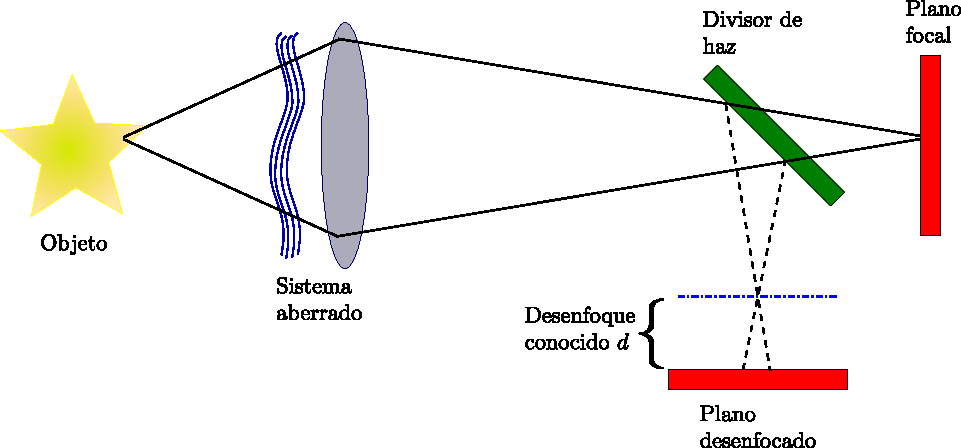
\includegraphics[scale=0.5]{img/pd.pdf}
		\end{frame}


		\begin{frame}
		\frametitle{Planteamiento del problema}
			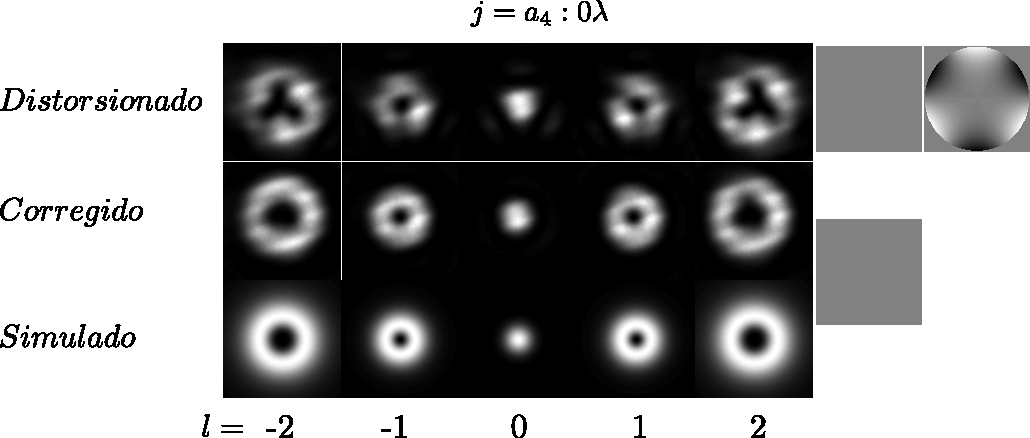
\includegraphics[scale=0.65]{img/exp_res_correction.pdf}
		\end{frame}		


	%%% Objetivos %%%
	\subsection{Objetivos}	
		\begin{frame}
		\frametitle{Objetivos}
		%\subsubsection{General}
			\begin{block}{Objetivo General}
			\justifying Solucionar la indeterminación que hay entre las aberraciones provenientes de la no idealidad de un modulador espacial de luz (SLM) y las aberraciones propias de un sistema óptico, al usar los algoritmos de diversidad de fase desarrollados por el grupo de óptica aplicada.
			\end{block}
			
		%\subsubsection{Específicos}
			\begin{block}{Objetivos Específicos}
				\begin{itemize}
				\justifying
				\item Implementar un algoritmo de PD que basado en imágenes sintéticas simule los efectos de modulación no lineal de un SLM. 
				\item Emplear la implementación anterior comparando con imágenes experimentales, con miras a encontrar las aberraciones causadas por fuentes diferentes a la modulación no lineal del SLM.
				\item Establecer si a partir de la combinación de los resultados de los objetivos anteriores puede reconstruirse la aberración del frente de onda obtenido con PD coherente.
				\item Validar experimentalmente los resultados obtenidos recuperando la fase de un objeto cuya aberración sea conocida.
				\end{itemize}
			\end{block}
			\end{frame}

		%		\begin{frame}
%		\frametitle{Planteamiento del problema}
%			En el trabajo presentado se propuso solucionar la indeterminación que hay al emplear algoritmos de diversidad (PD) de fase para la detección de aberraciones causadas por sistema ópticos, ya que en dichos algoritmos no es posible distinguir la contribución a las aberraciones causadas por la modulación en fase de un modulador espacial de luz (SLM) y los demás elementos ópticos.
%		\end{frame}

	%%% Planteamiento del problema %%%
	%\subsection{Aplicaciones de los OVs}	
		\begin{frame}
		\frametitle{Aplicaciones de los vórtices ópticos:\\-Microscopía de fase}
				\begin{center}
				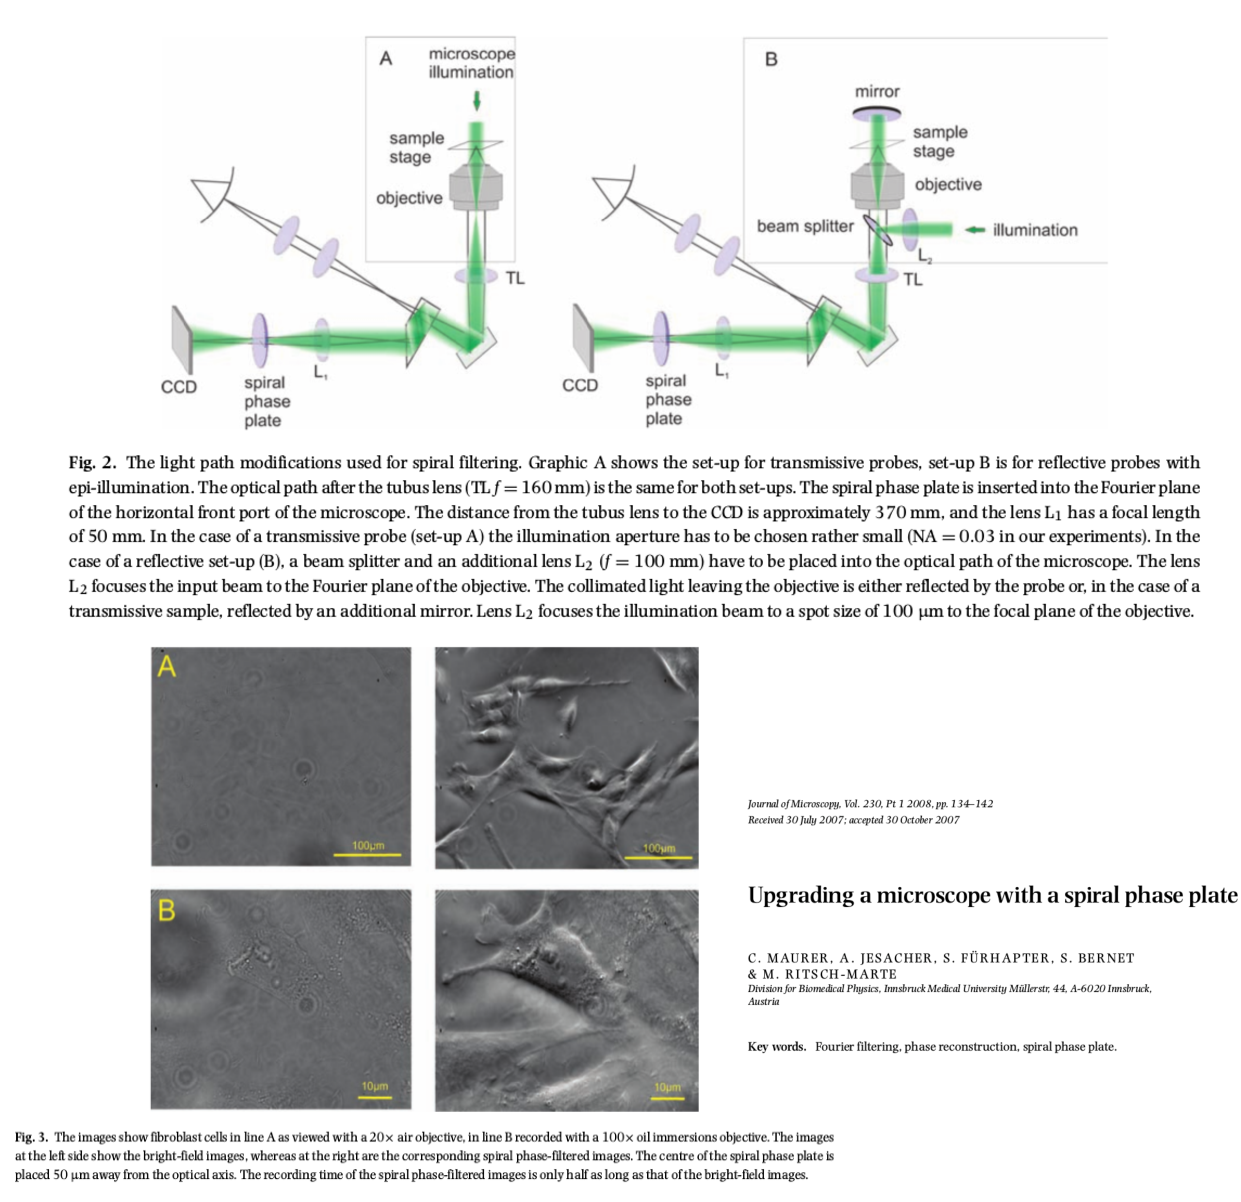
\includegraphics[scale = 0.4, keepaspectratio]{img/micro.pdf}
				\end{center}
%		\caption{A) Vórtice óptico, B) perfil de fase azimutal $\theta(x,y)$ y C) propagación de la fase.}
		\end{frame}
		
%	\subsection{- Transmisión de información}	
		\begin{frame}
		\frametitle{Aplicaciones de los vórtices ópticos:\\ -Transmisión de información}
				\centering
				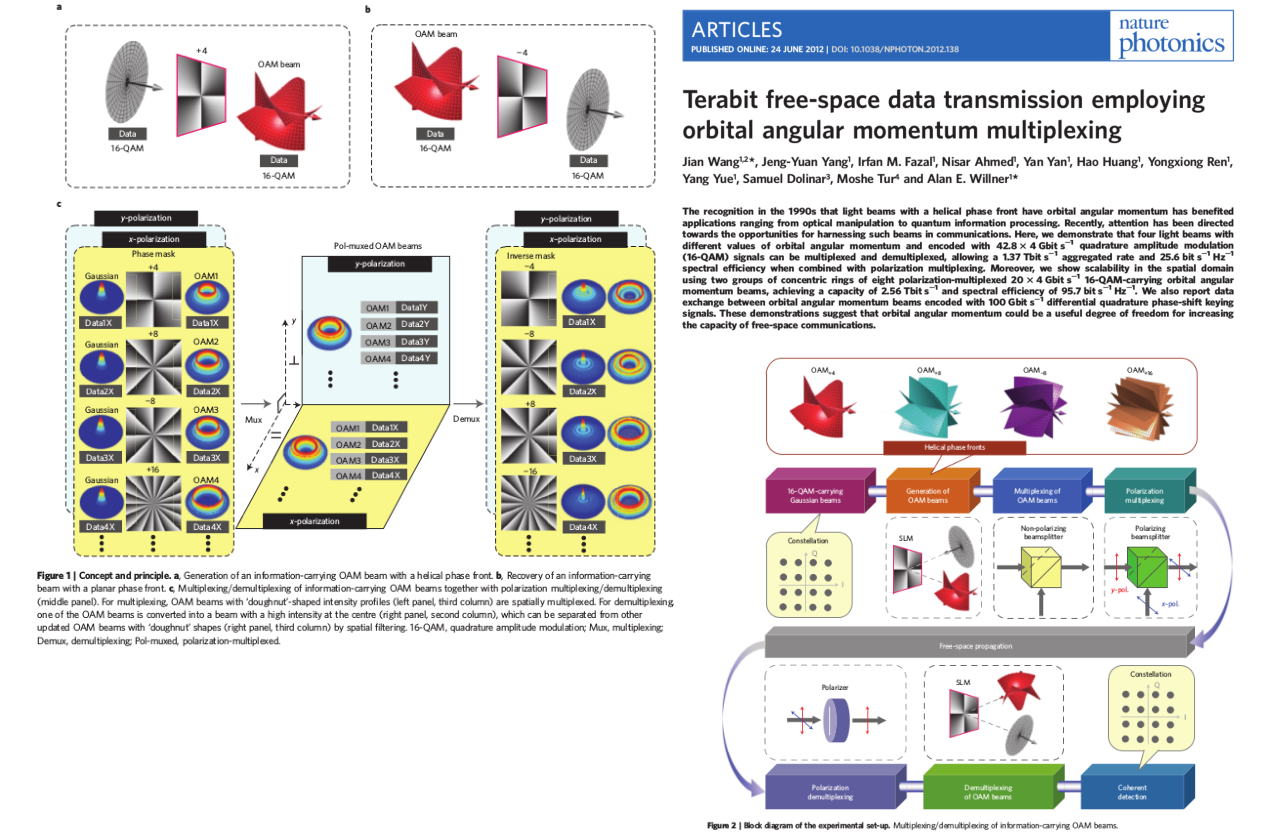
\includegraphics[scale=0.5]{img/Transmision.pdf}
%		\caption{A) Vórtice óptico, B) perfil de fase azimutal $\theta(x,y)$ y C) propagación de la fase.}
		\end{frame}
		
		\begin{frame}
		\frametitle{Aplicaciones de los vórtices ópticos:\\ -Pinzas ópticas}
				\centering
				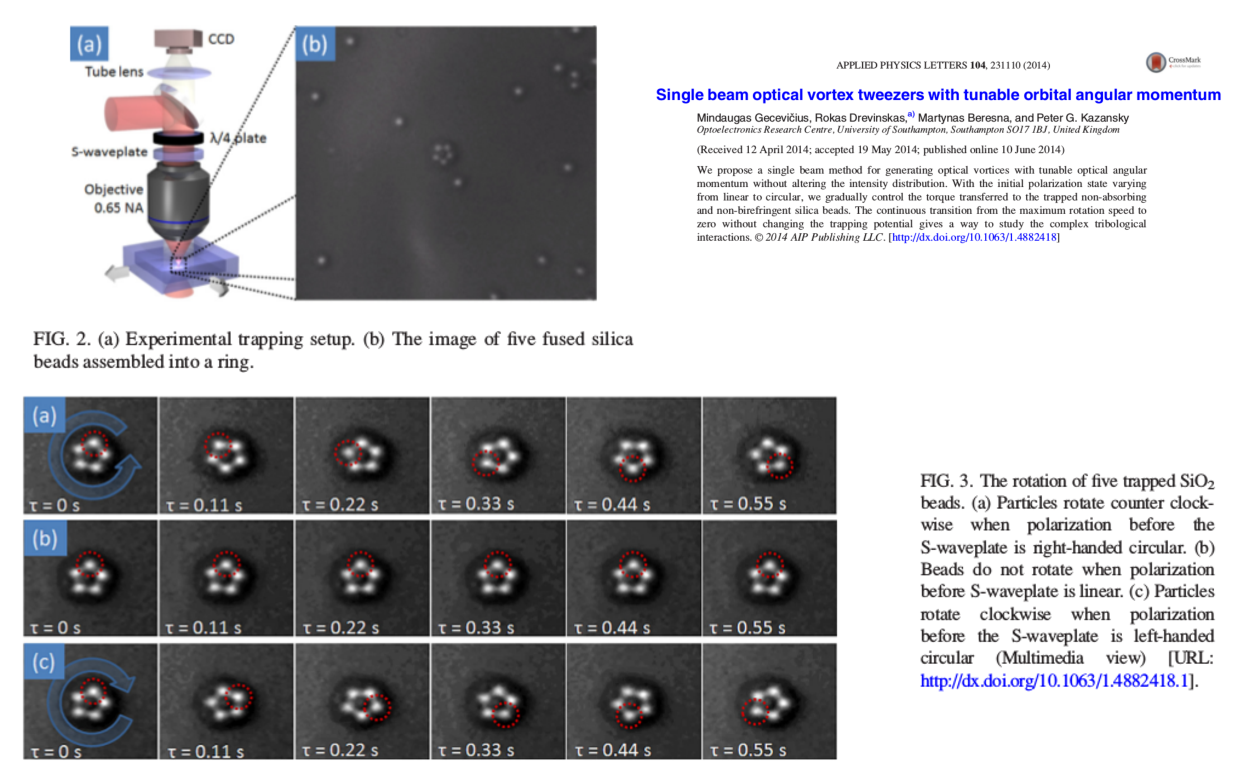
\includegraphics[scale=0.5]{img/tweezers.pdf}
%		\caption{A) Vórtice óptico, B) perfil de fase azimutal $\theta(x,y)$ y C) propagación de la fase.}
		\end{frame}
		
%		\subsection{Aplicaciones de PD}			

		
		\begin{frame}
		\frametitle{Aplicaciones de diversidad de fase:\\ -Óptica adaptativa}
			\begin{center}
				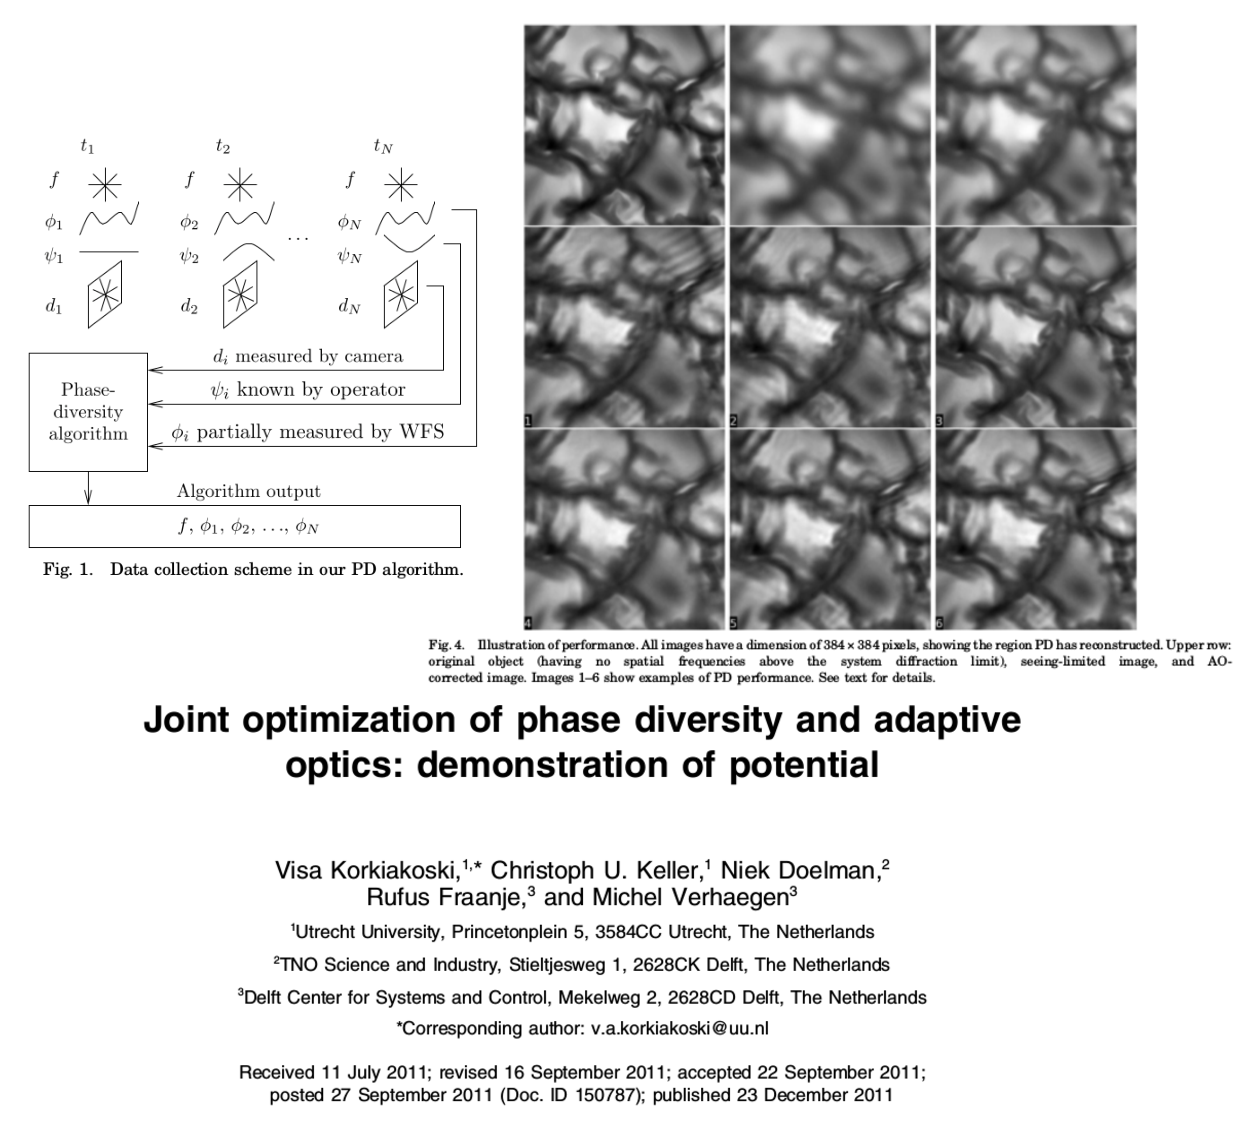
\includegraphics[scale=0.4]{img/PDAO.pdf}
			\end{center}
%		\caption{A) Vórtice óptico, B) perfil de fase azimutal $\theta(x,y)$ y C) propagación de la fase.}
		\end{frame}
		
		\begin{frame}
		\frametitle{Aplicaciones de diversidad de fase:\\ -Sensor de frente de onda}
			\begin{center}
				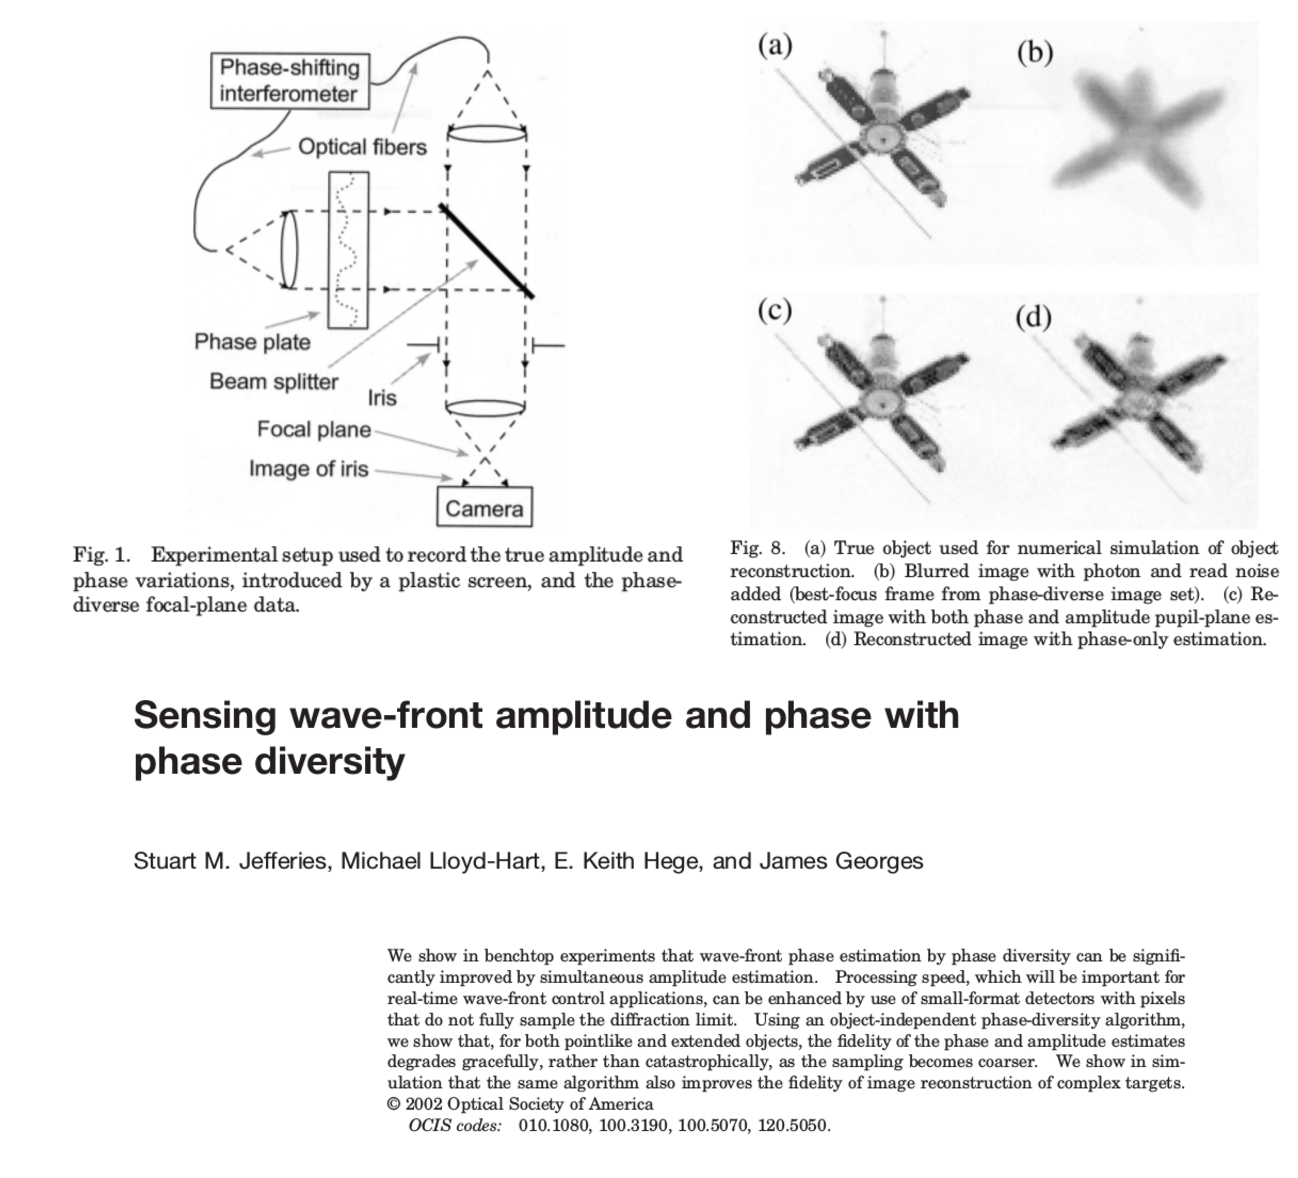
\includegraphics[scale=0.4]{img/PDWFS.pdf}
			\end{center}
%		\caption{A) Vórtice óptico, B) perfil de fase azimutal $\theta(x,y)$ y C) propagación de la fase.}
		\end{frame}
		


	
	%%% Justificación %%%
%	\subsection{Justificación}
%		\begin{frame}
%		\frametitle{Justificación}
%			No sé cómo y si ponerla prob. si
%		\end{frame}
				
\section{Generación de vórtices ópticos}
	\setcounter{subsection}{1}				

	\subsection{Marco teórico}
		%\subsection{Vórtices ópticos}
	
		%%%% OV: Introducción %%%%
		%%%% OV: Definición %%%%		
%		\begin{frame}
%		\frametitle{Vórtice óptico}
%Un vórtice óptico (VO) es una dislocación del frente de onda que genera una singularidad en la fase y causa un punto de intensidad nula. 
%		\footnote{M. R. Dennis, K. O’Holleran, and M. J. Padgett. ``Chapter 5 singular optics: Optical vortices and polarization singularities''. Progress in Optics, volumen 53, páginas 293–363. Elsevier, 2009.} 
%		
%		Su función de onda depende de la distribución espacial del frente de onda de forma que la fase es proporcional al plano azimutal
%		\begin{equation}
%		\psi(x,y) \propto e^{qi\theta(x,y)},
%		\end{equation}
%		donde $q$ es un entero conocido como carga topológica y, 		$$\theta(x,y) = \arctan\left(\frac{y}{x}\right)$$
%		\begin{figure}
%		\includegraphics[scale=0.3]{img/dibujo.png}
%		\caption{A) Vórtice óptico, B) perfil de fase azimutal $\theta$ y C) propagación de la fase.}
%		\end{figure}	
%		\end{frame}		
		%%%% OV: Generación %%%%
		\begin{frame}
		
		\frametitle{Marco teórico: Generación de vórtices ópticos}
\begin{multicols}{3}
			\vfill
			\centering Manipulación controlada de las propiedades de los láseres\footnote{T. Ohtomo, S. Chu, and K. Otsuka. ``Generation of vortex beams from lasers with controlled herte- and ince- gaussian modes''. Optics Express, \textbf{16}(7), 5082–5094 (2008).}.
%			\begin{figure}
			\vspace*{30pt}\includegraphics[scale=0.25]{img/LGmodos.pdf}
%			\caption{Modos Laguerre-Gauss}
%			\end{figure}
			\vfill
			
			\newpage
			\vfill
			\centering Empleando placas espirales de fase (SPP)\footnotemark[1]. 
%			\begin{figure}
			\includegraphics[scale=0.25
			]{img/SPP.eps}
%			\caption{VO a partir de SPP. }
%			\end{figure}
			
			\newpage 
			\vfill
			\centering Empleando redes de difracción\footnotemark[1].
%			\begin{figure}
			\includegraphics[scale=0.25]{img/DiffGrat.eps}
%			\caption{VO a partir de redes de difracción.}
%			\end{figure}
		\end{multicols}
		
		\end{frame}	

		%%%% OV: SLMs %%%%
		\subsection{Modulador espacial de luz}
		\begin{frame}
		\frametitle{Modulador espacial de luz}
		Dispositivos que modulan amplitud o fase de ondas de luz en espacio y tiempo\footnote{HOLOEYE Photonics. \url{http://holoeye.com/spatial-light-modulators/}}.
		

%		\begin{figure}
%		\begin{columns}
%		\column{0.6\textwidth}
		\begin{columns}
		\column{0.7 \textwidth}
		\centering
		\includegraphics[scale=0.4]{img/Mod.eps}
%		\caption{Moduladores espaciales de luz.\footnotemark[3]}
%		\end{figure}
		\column{0.3 \textwidth}
		\centering
		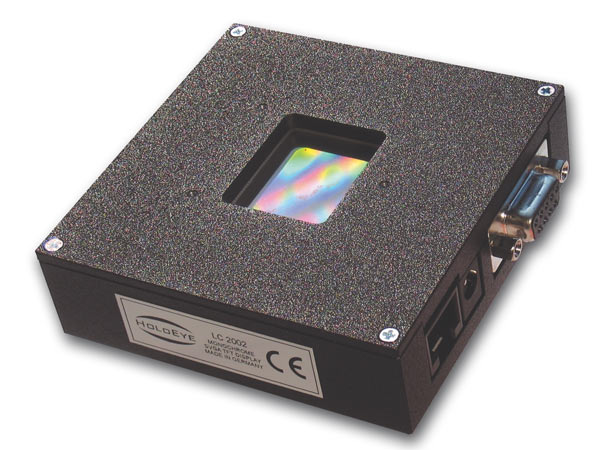
\includegraphics[scale=0.15]{img/lc2002.jpg}
		\end{columns}
		\begin{center}
		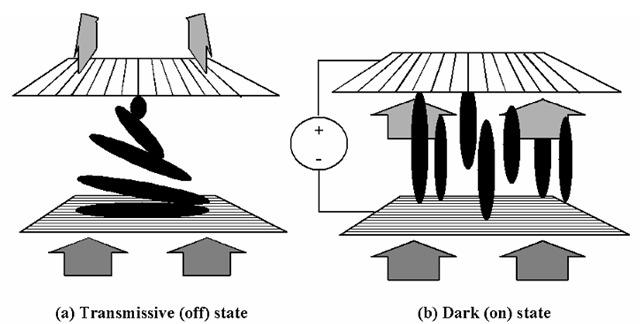
\includegraphics[scale=0.20]{img/tnlcd.png}\\
		\tiny Imagen tomada de \url{http://what-when-how.com/wp-content/uploads/2012/06/tmp7ee150_thumb2.png}		
		\end{center}	
		\end{frame}	

%%\setbeamertemplate{logo}{}
%%\setbeamertemplate{logo}{
\includegraphics[scale=0.15]{logoeafit.png}\vspace{0pt}}

		\setbeamertemplate{logo}{}
		
		\subsection{Caracterización de las curvas de modulación}
		\begin{frame}
		\frametitle{Caracterización de la curva de modulación}
		\centering
		\hspace*{-10pt}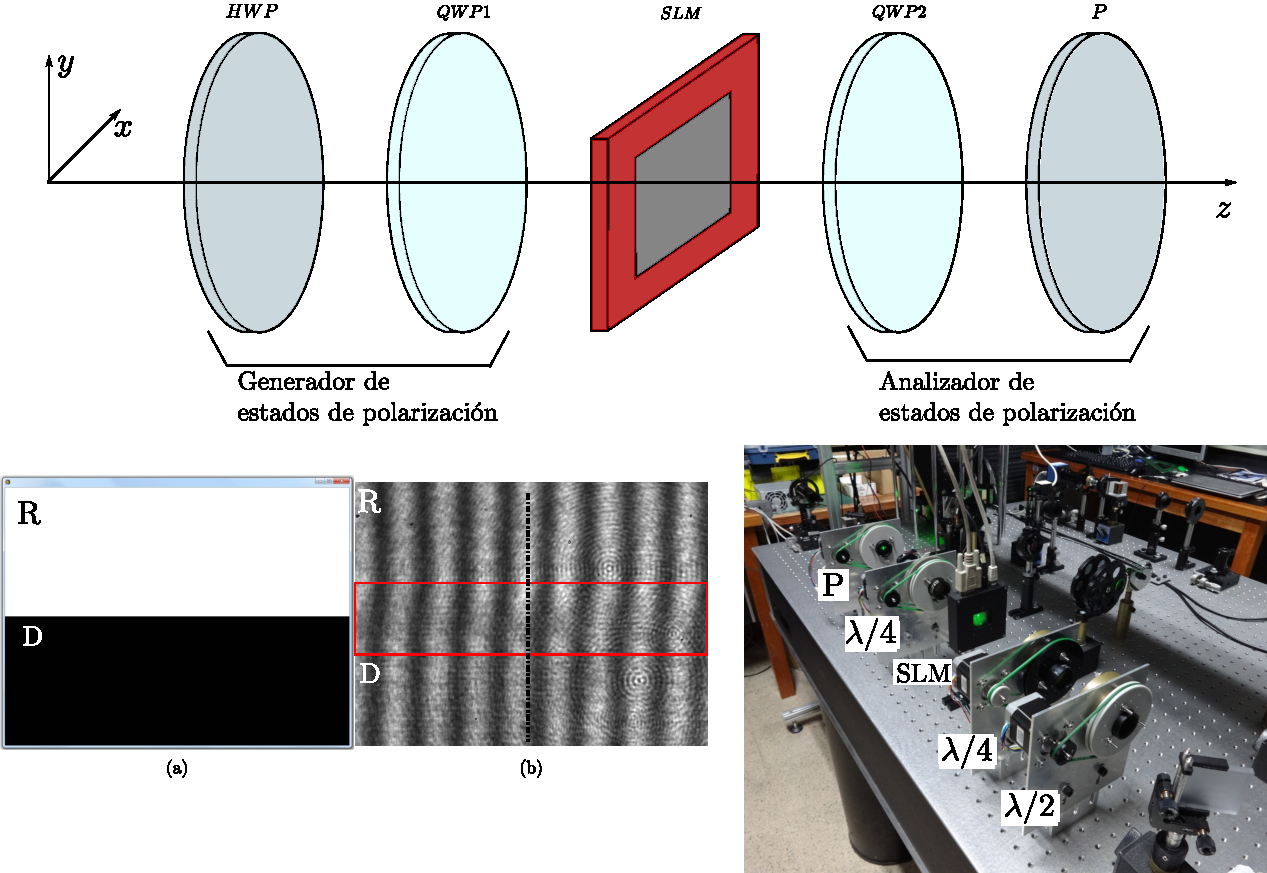
\includegraphics[scale=0.54]{img/CarMod.pdf}
%		\vspace{10pt}
%		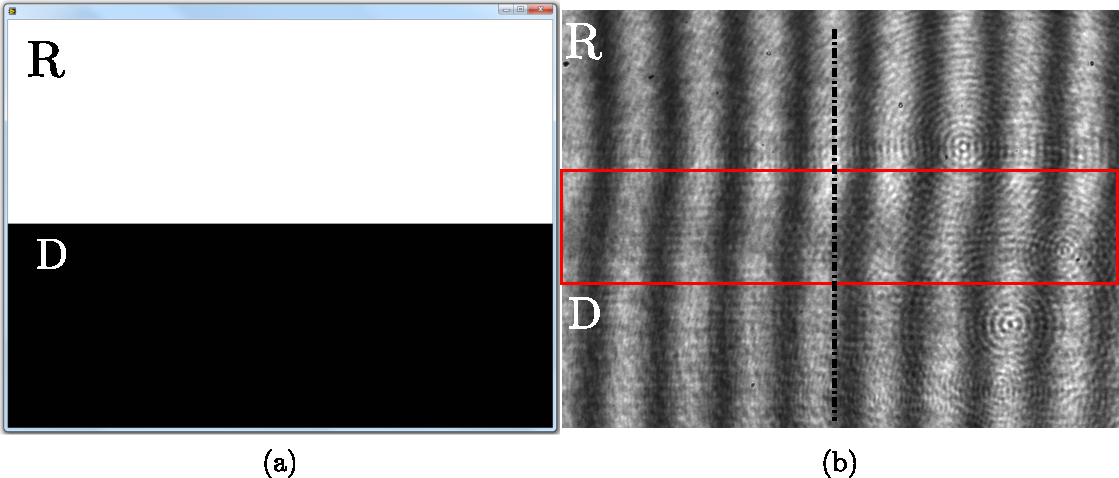
\includegraphics[scale=0.5]{img/faseslm.pdf}
		%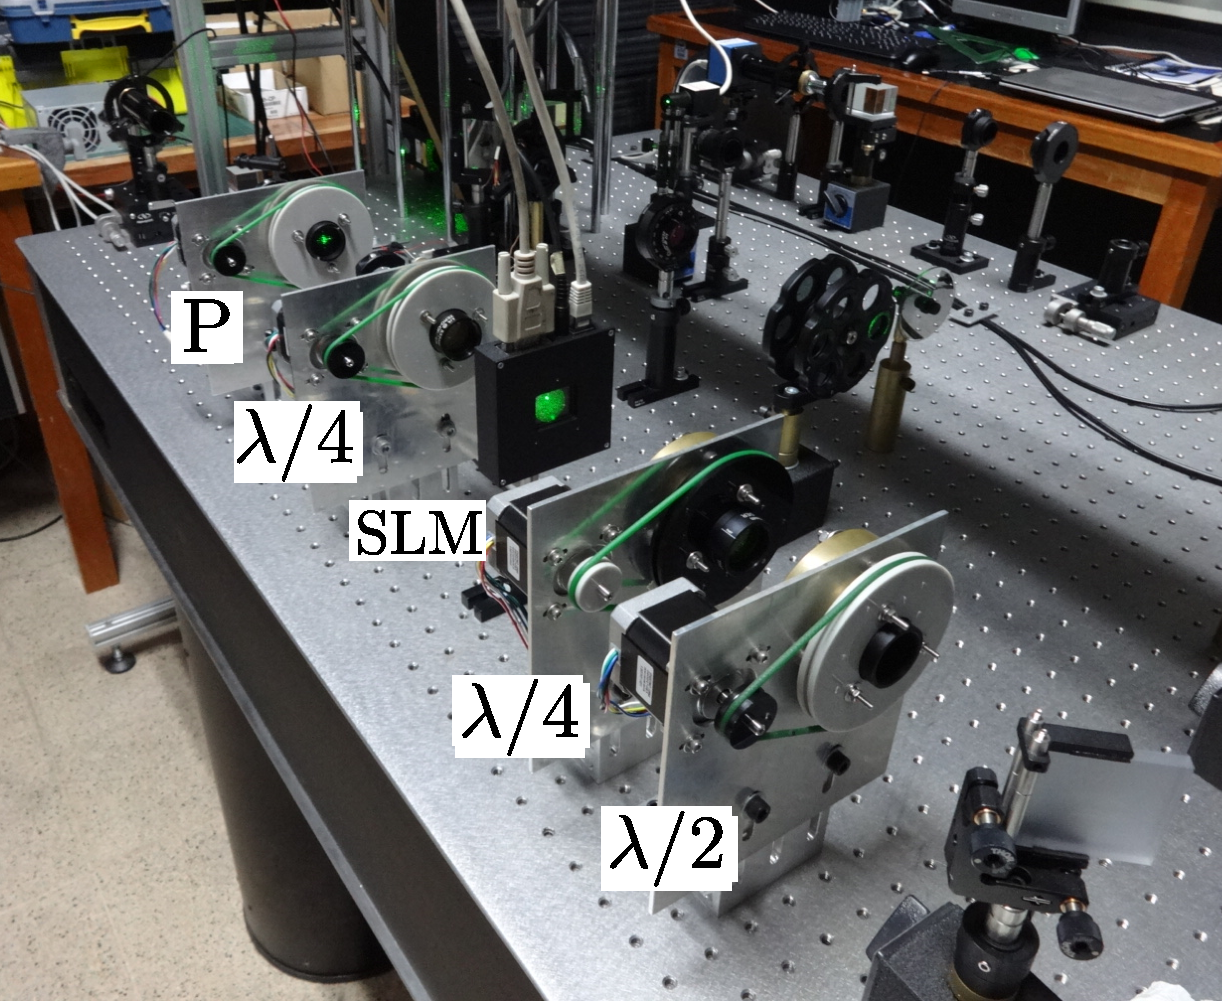
\includegraphics[scale=0.4]{img/rotadores.pdf}
		\end{frame}
		\setbeamertemplate{logo}{
\includegraphics[scale=0.12]{img/logoeafit.png}\vspace{0pt}}
		
		
%		\subsection{Resultados: Caracterización del SLM}
		\begin{frame}
		\frametitle{Resultados: Curvas de modulación}
		\centering
		\hspace*{-20pt}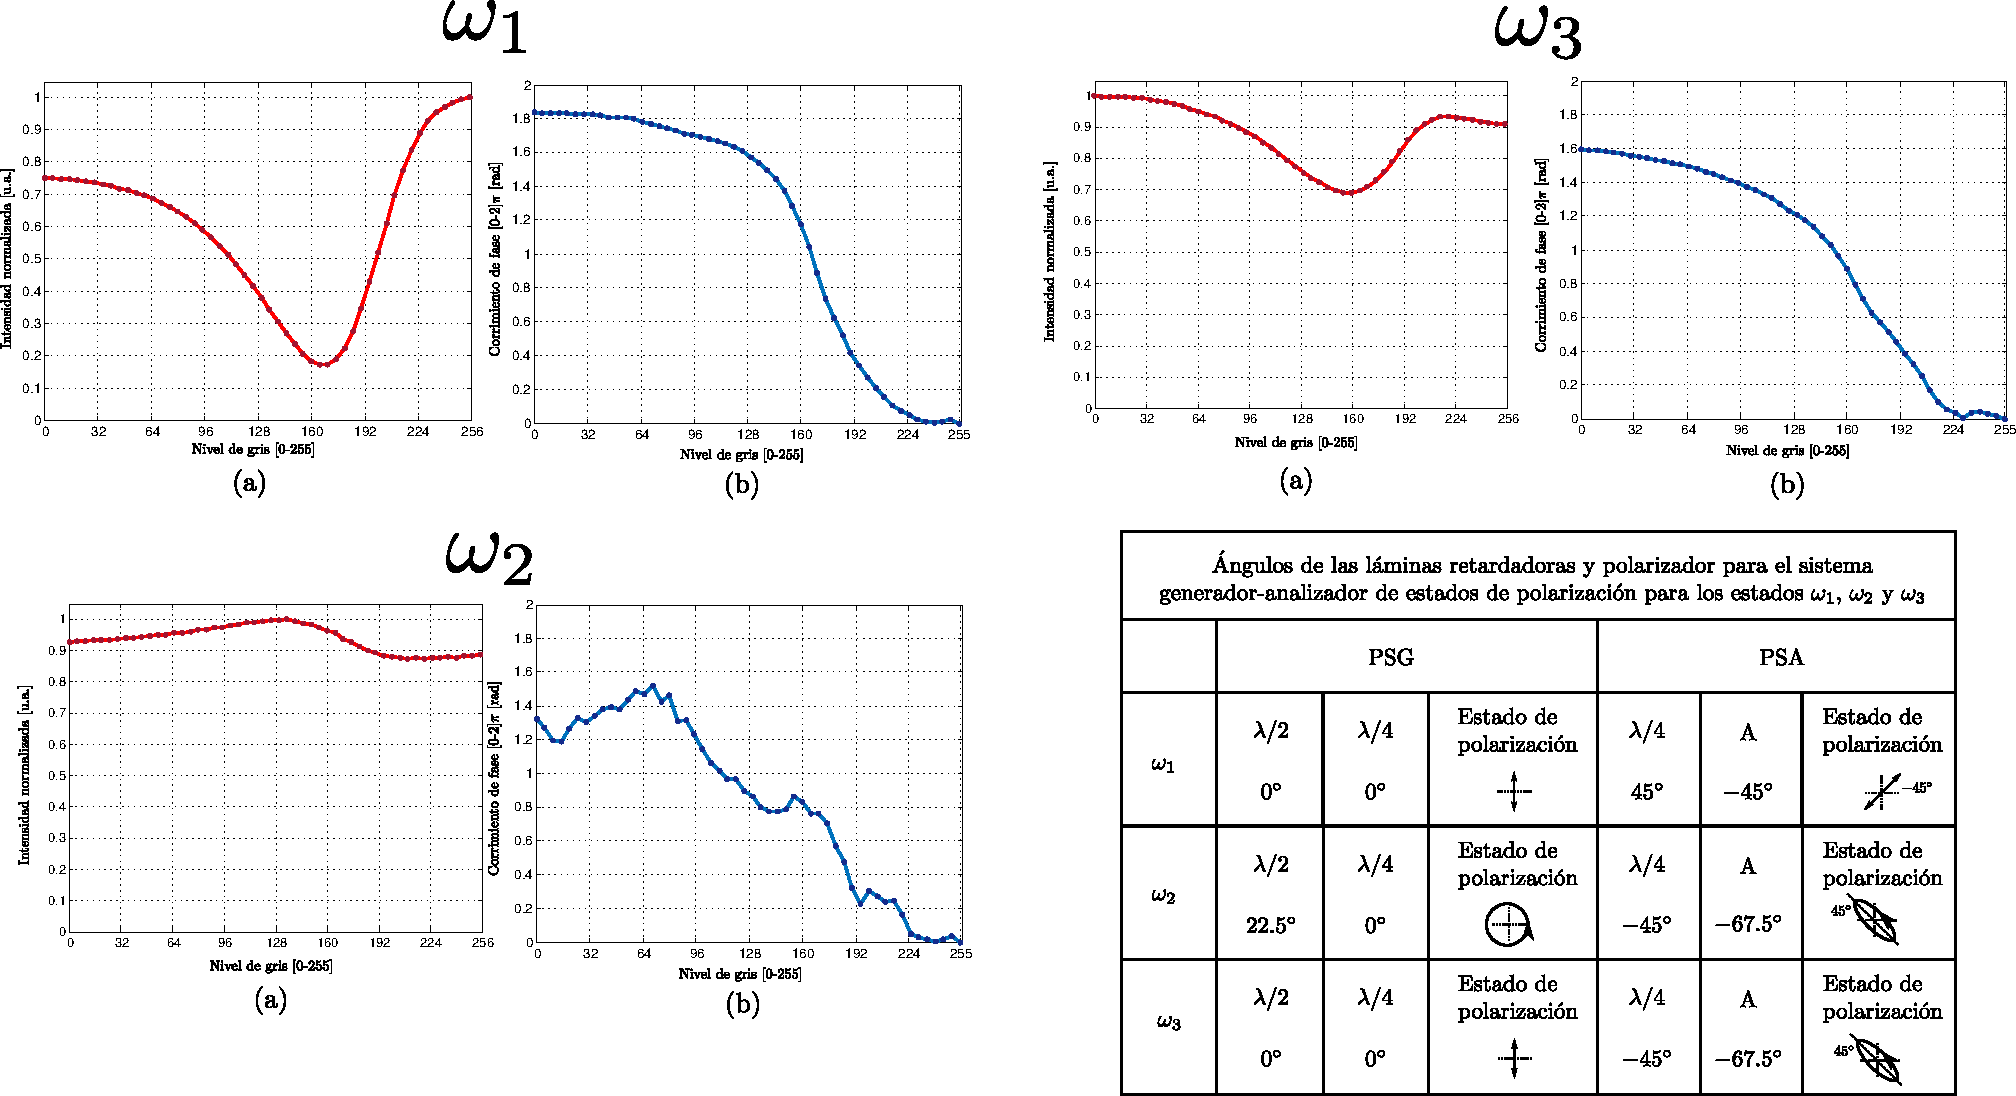
\includegraphics[scale=0.35]{img/curvas.pdf}
		\end{frame}

		\begin{frame}
		\frametitle{Una plataforma para la generación de máscaras}
		\begin{center}
		\hspace*{-15pt}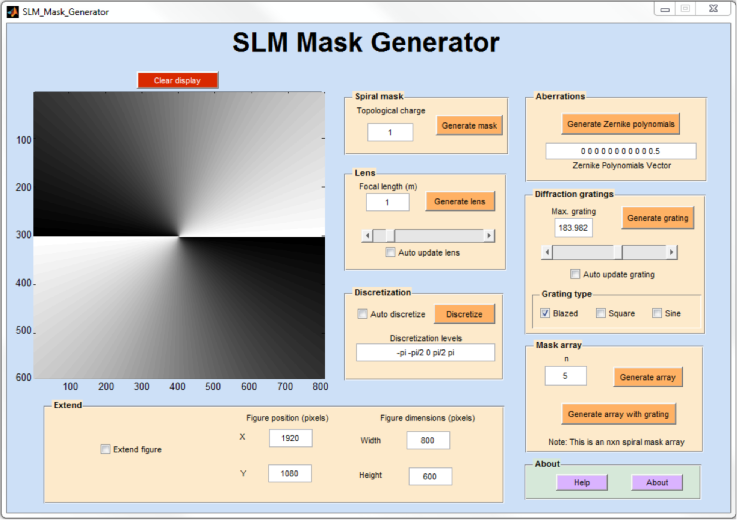
\includegraphics[scale=0.4]{img/maskgen.png}
		\end{center}
		\end{frame}				
		
		\begin{frame}
		\frametitle{Resultados: Generación de OVs a partir de las curvas de modulación}
%		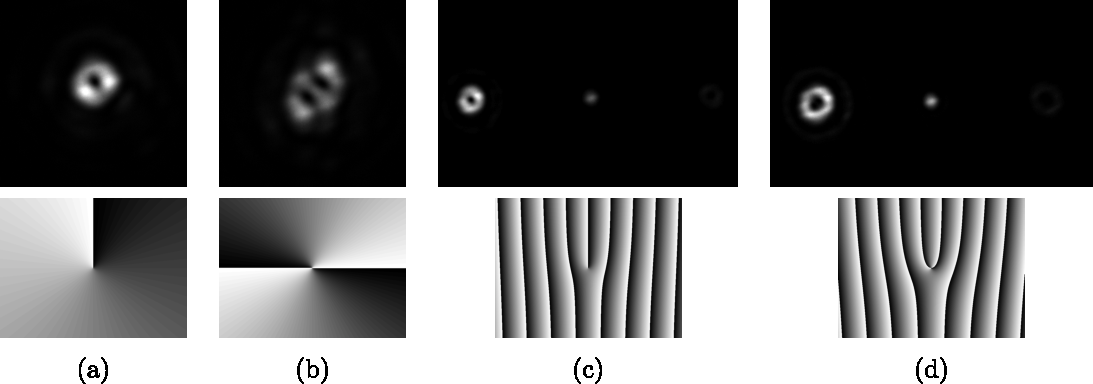
\includegraphics[scale=0.5]{img/resmaskapp.pdf}
%		\vspace{10pt}
		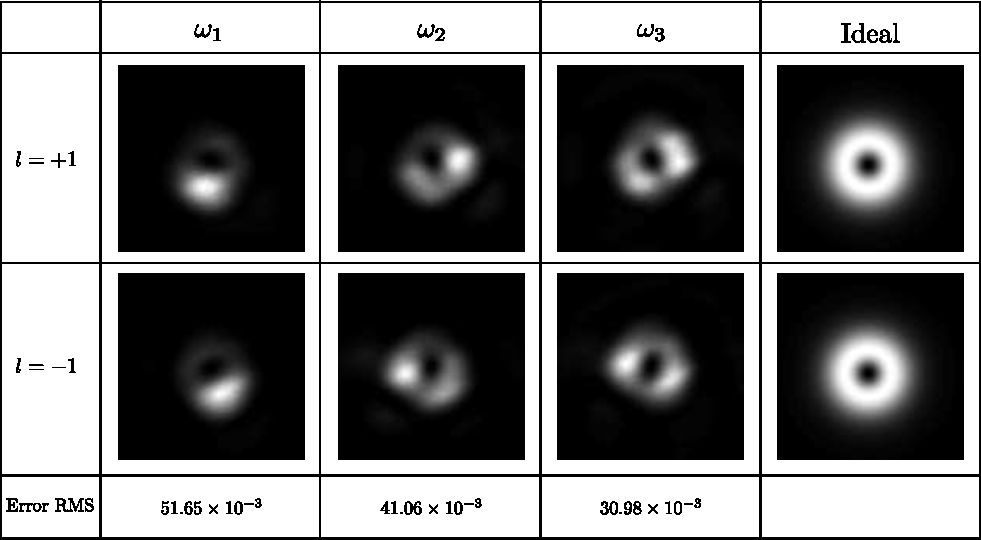
\includegraphics[scale=0.65]{img/ovcurvas.pdf}\\
		$$E = \sqrt{\frac{1}{MN} \sum\limits_{n,m}^{M,N} |d-u|^2}$$
		\end{frame}
		
		
		\subsection{Aberraciones en vórtices ópticos}
		\begin{frame}
		\frametitle{Aberraciones en vórtices ópticos}
		
		\begin{multicols}{2}
		Pueden provenir de imperfecciones en: 
			\begin{itemize}
			\item diseño,
			\item los materiales,
			\item alineación de los elementos ópticos.
			\end{itemize}
			
		\newpage
		\justifying
			En nuestro caso, también por características no deseadas causadas por  el SLM, tales como el acople entre la modulación en fase y amplitud, factor de llenado y la discretización.

		\end{multicols}

%		\begin{figure}
		\centering
		\includegraphics[scale=0.35]{img/ovsimreal.pdf}
%		\caption{Efectos de modulación no ideal sobre VO.}
%		\end{figure}
		
		\end{frame}		
		
		\begin{frame}
		\frametitle{Simulación de los efectos de la modulación no ideal en OVs}
		\begin{center}
		 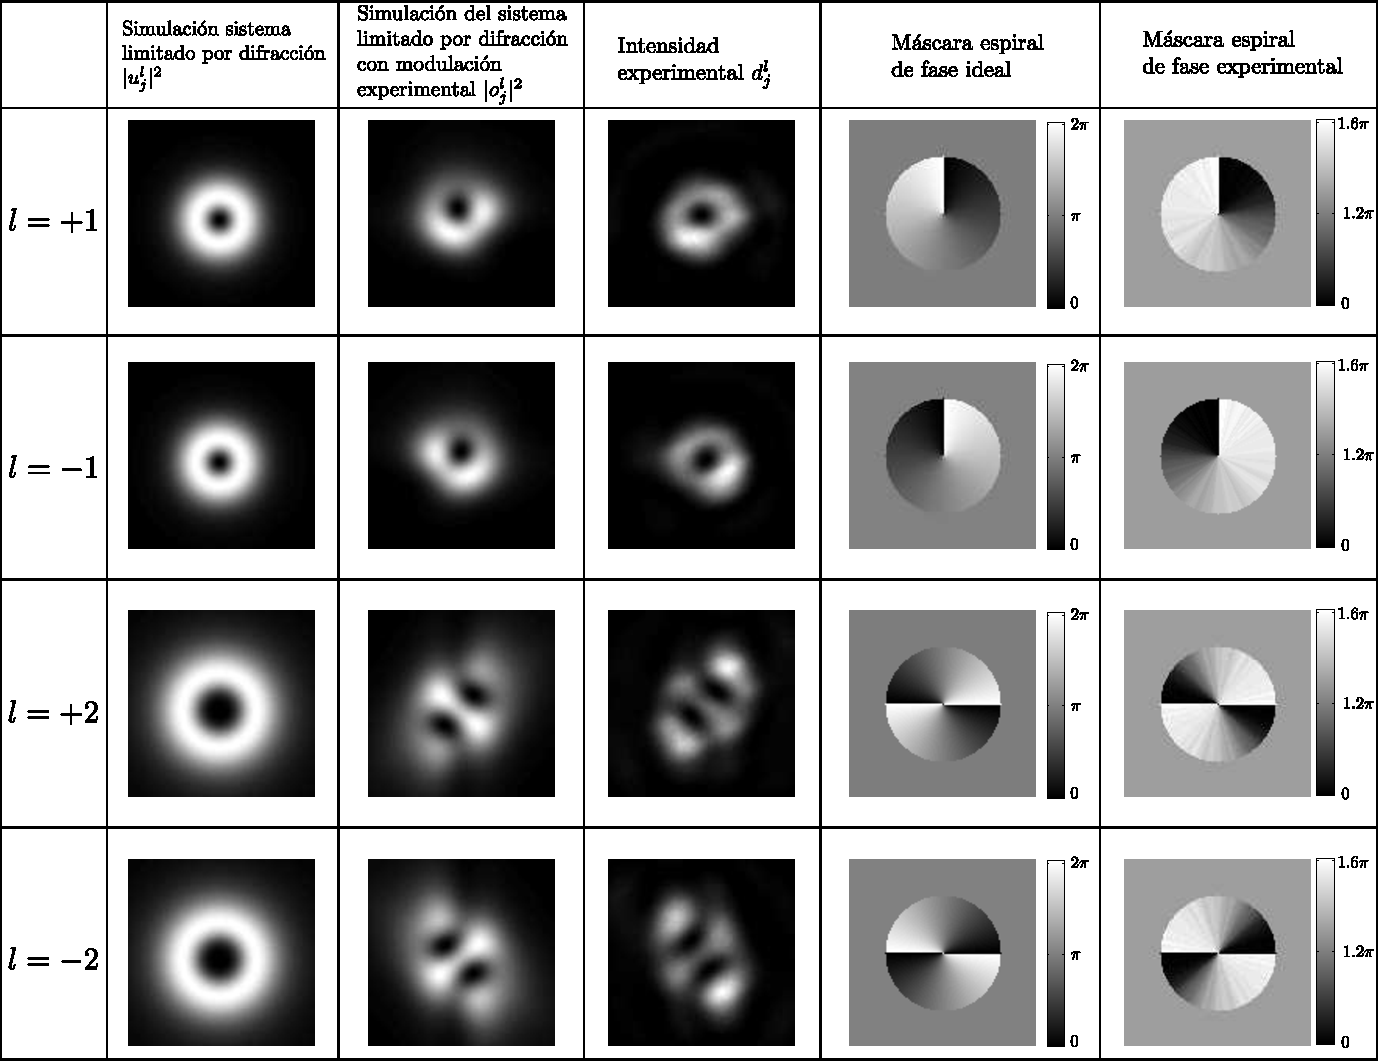
\includegraphics[scale=0.4]{img/SimOVExp.pdf}
		 \end{center}
		\end{frame}
				
				
%%%%%%%%%%%% AQUI TERMINAN LOS VÓRTICES ÓPTICOS %%%%%%%%%%%%%%
				

\section{Caracterización de aberraciones en vórtices ópticos}
	\setcounter{subsection}{1}
	
		%%% PD: Introducción %%%
		\begin{frame}
		\frametitle{Cómo se caracterizan las aberraciones?}
			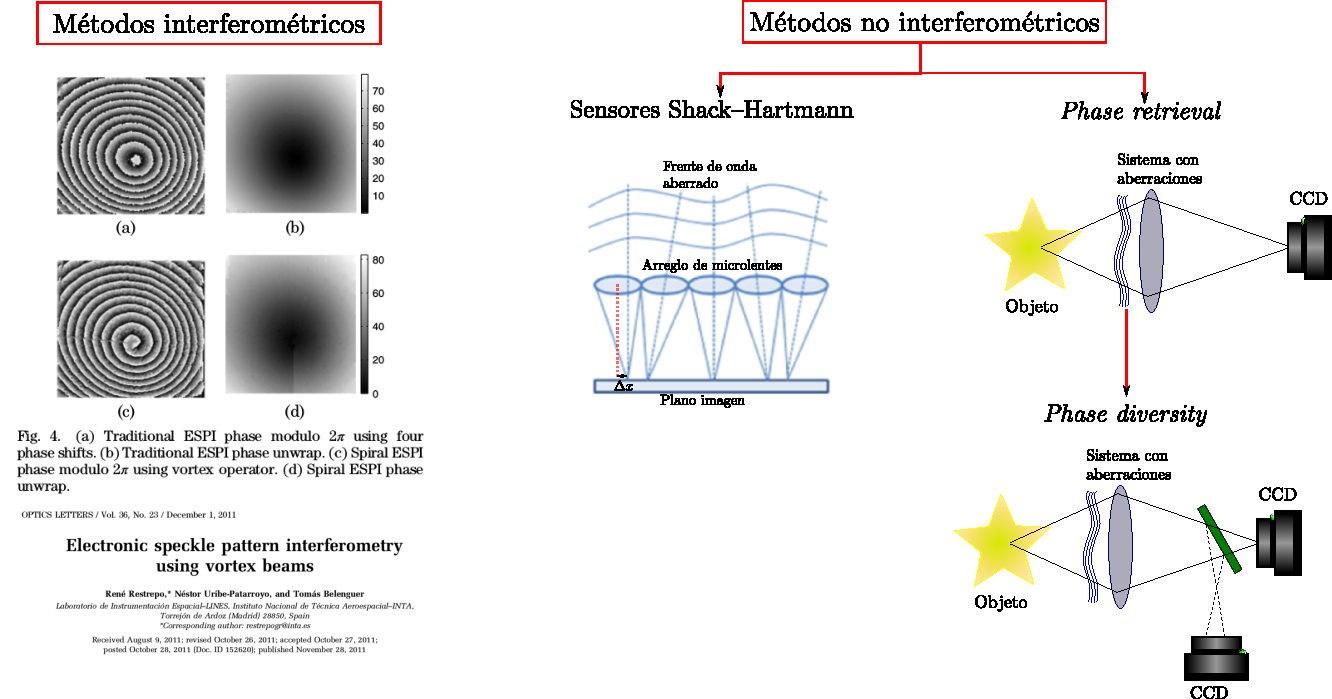
\includegraphics[scale=0.5]{img/WFS.pdf}
		\end{frame}
		
		\subsection{Marco teórico}
		%%% PD: Introducción %%%
		\begin{frame}
		\frametitle{Marco teórico: Sistemas formadores de imagen}

		\begin{multicols}{2}
		\justifying Las técnicas de \textit{phase retrieval} analizan el efecto de las aberraciones sobre las imágenes que produce un sistema óptico. Las aberraciones son caracterizadas cuando se encuentra una función de transferencia que
reproduce las imágenes registradas.

		\newpage
		\vspace*{10pt}
		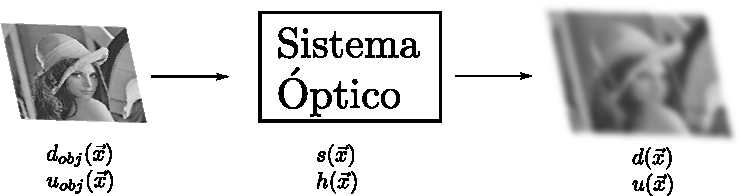
\includegraphics[scale=0.45]{img/sisforim.pdf}
		\end{multicols}
		\vspace{10pt}
		
		\hspace*{-20pt}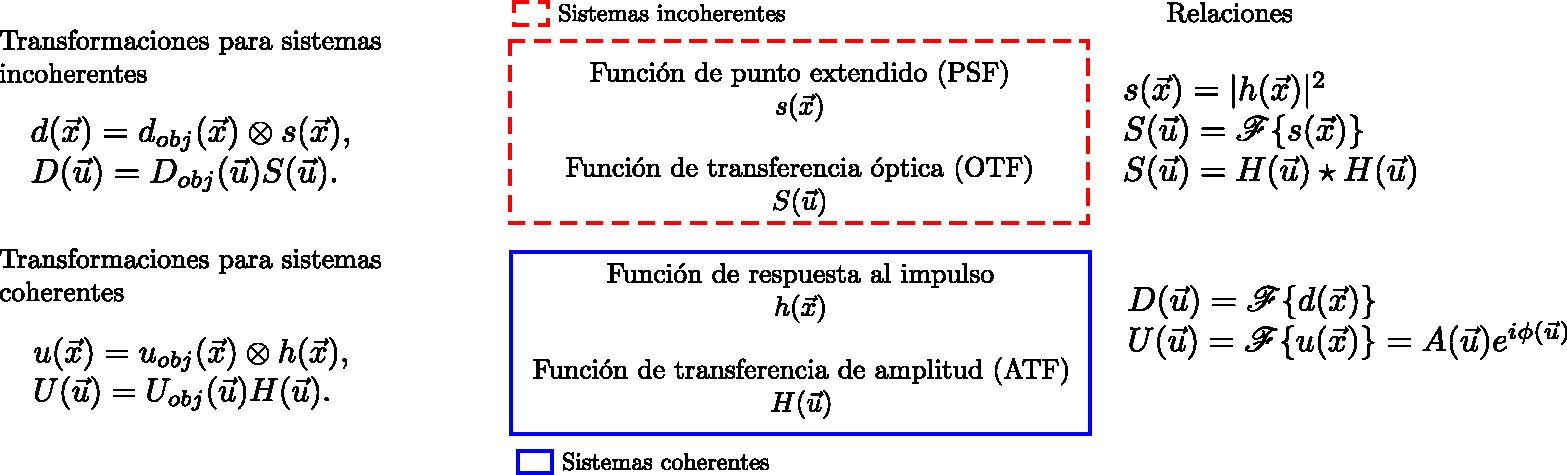
\includegraphics[scale=0.45]{img/Transformaciones.pdf}

		\end{frame}
		
		\subsection{Diversidad de fase}
		
		\setbeamertemplate{logo}{}
		\begin{frame}
		\frametitle{Diversidad de fase}
		\vspace*{20pt}
		\begin{multicols}{2}
		
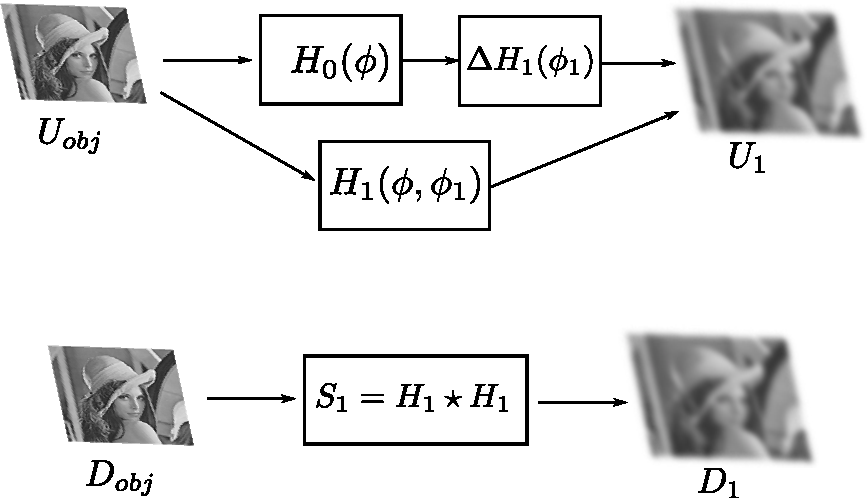
\includegraphics[scale=0.55]{img/PDFun.pdf}
		
		\newpage
		
		\hspace*{100pt}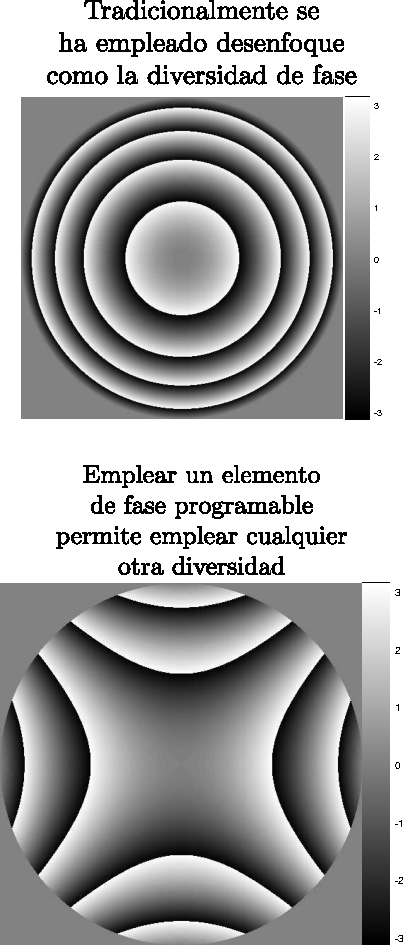
\includegraphics[scale=0.3]{img/diversidades.pdf}
		
		\end{multicols}		
		
		\vspace{10pt}
		\begin{block}{\centering Funcional de minimización}
			\centering
			$L(\overline{D}_{obj}, \phi) = \sum\limits_{j=0}^K \sum\limits_{m,n}^{M,N} |D_j - \overline{D}_{obj} S_j|^2.$
		\end{block}
		\end{frame}


		\begin{frame}
		\frametitle{Diversidad de fase con iluminación coherente}
		
		\vspace*{20pt}
		
		\begin{multicols}{2}

		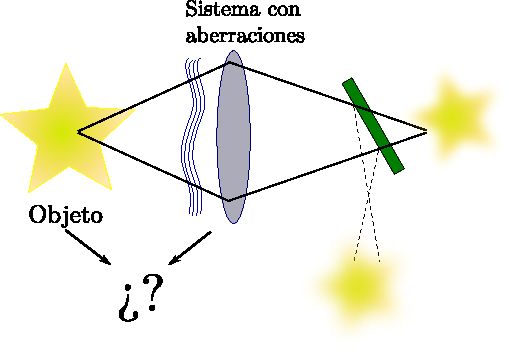
\includegraphics[scale=0.65]{img/objetopd.pdf}

		\newpage
		\centering
		En el laboratorio podemos escoger el tipo de iluminación y definir nuestro campo objeto $u_{obj}$\\
		\vspace*{15pt}
		$ u_{obj} = \exp \left( \frac{-(x^2+y^2)}{\sigma} \right) $\vspace*{30pt}
		
		$u_j(\vec{x}) = \mathscr{F}^{-1} \{ U_{obj}H(\vec{u}) H_j(\vec{u})\} $
		\end{multicols}
		\vspace*{30pt}
		\begin{block}{\centering Un nuevo funcional de minimización}
			\centering
			$L(\phi) = \sum\limits_{j=0}^K \sum\limits_{m,n}^{M,N} |d_j - |u_j|^2|^2.$
			\end{block}
			
		\end{frame}
		
		\begin{frame}
		\frametitle{PD con iluminación coherente mejorado con vórtices ópticos.}
		
		\begin{columns}
		\column{0.6\textwidth}
		\begin{block}{\centering Una nueva familia de diversidades}
		\centering
		$\psi_l = \exp \{il\theta\},$\\
		\vspace*{10pt}
		$u_{j}^l (\vec{x}) = \mathscr{F}^{-1} \{U_{obj}(\vec{u}) H(\vec{u}) \Delta H_j(\vec{u}) \psi_l (\vec{u})\}.$
		
		\end{block}
		
		\column{0.4\textwidth}		
		\begin{block}{\centering  Funcional extendido}
		\centering
		$L(\phi) = \sum\limits_{l=0}^{L} \sum\limits_{j=0}^{K} \sum\limits_{m,n}^{M,N} |d_j^l - |u_j^l|^2|^2.$
		\end{block}
		\end{columns}		
		\vspace*{10pt}
		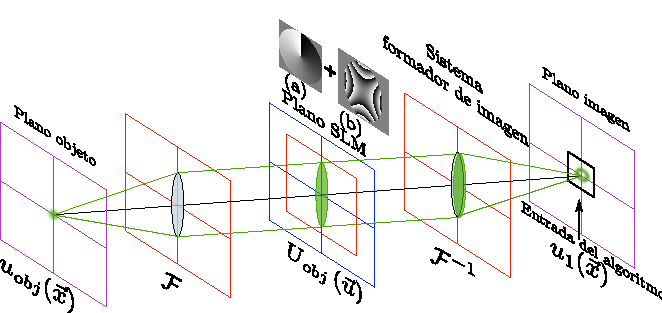
\includegraphics[scale=1]{img/montaje_dibujo.pdf}
		\end{frame}

\setbeamertemplate{logo}{
\includegraphics[scale=0.12]{img/logoeafit.png}\vspace{0pt}}

		%%% PD: PD coherete %%%
		\begin{frame}
		\frametitle{Diagrama de flujo de diversidad de fase coherente}
		\centering
			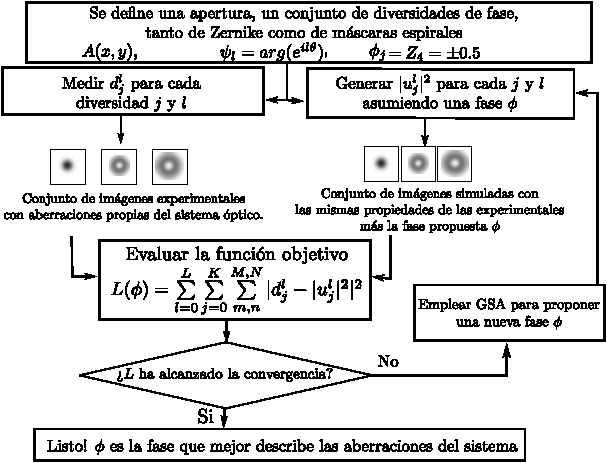
\includegraphics[scale=1]{img/PDflux.pdf}
		\end{frame}

			%%% Resultados corrección con PD coherente %%%
	\subsection{Corrección de aberraciones con diversidad de fase coherente}
		\begin{frame}
		\frametitle{Resultados: Corrección de aberraciones con diversidad de fase coherente}
		\begin{center}
		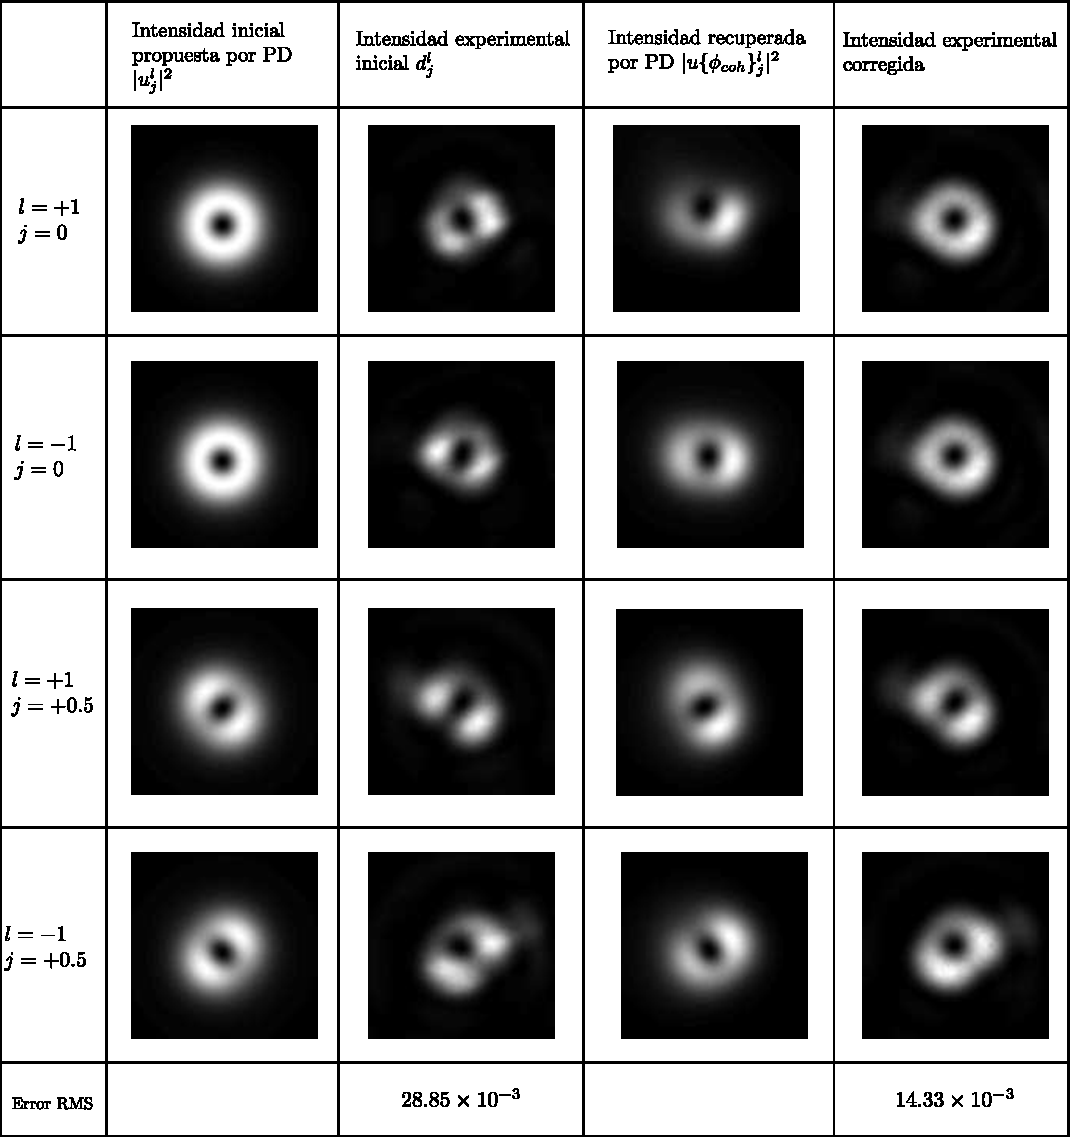
\includegraphics[scale=0.4]{img/CorPD0.pdf}
		\end{center}

		\end{frame}

		%%% PD: Modificaciones sobre PD coherente %%%
%		\begin{frame}
%		\frametitle{Corrección con PD coherente}
%			Aquí van los resultados de la corrección
%		\end{frame}
		%%% PD como sensor de aberraciones a causa de modulación en fase %%%
	%\subsubsection{Diversidad de fase como sensor de aberraciones a causa de la modulación en fase}
	
	\subsection{Modificaciones sobre diversidad de fase}
	
		\setbeamertemplate{logo}{}
			\begin{frame}
		\frametitle{Modificaciones sobre PD coherente}
			\begin{center}
			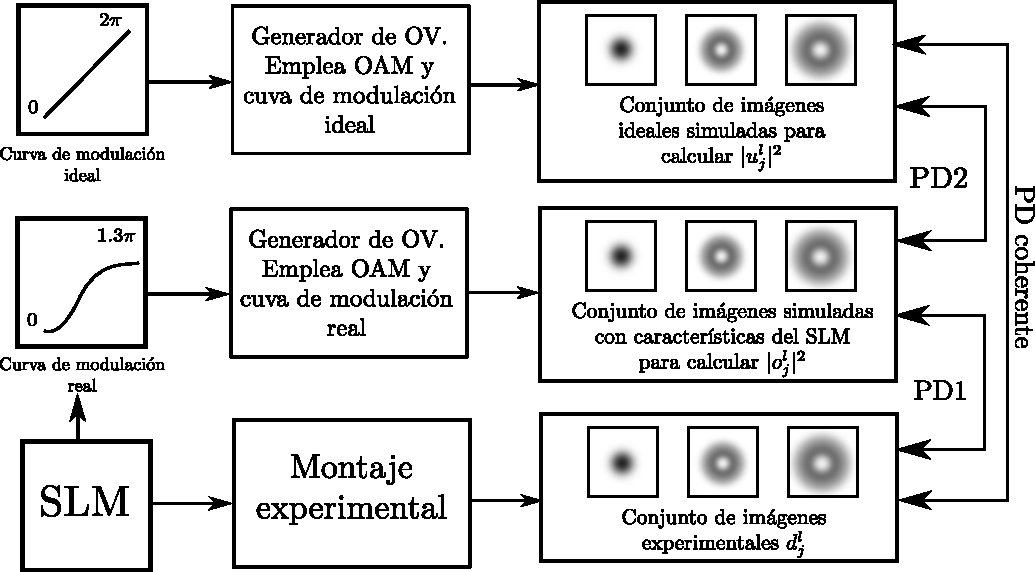
\includegraphics[scale=0.6]{img/PD012fulx.pdf}
			
			\begin{block}{\centering Nuevo funcional generalizado}
			\centering
			$ L(\phi) = \sum\limits_{l=0}^L \sum\limits_{j=0}^K \sum\limits_{u,v}^{M,N} |(d_j^l, |u_j^l|^2) - (|u_j^l|^2,|o_j^l|^2)|^2$
			\end{block}
			
	\end{center}
%			\begin{block}{Resumen }
%				\begin{tabular}{|c|p{8cm}|}
%	\hline 
%	PD coherente & Aberraciones globales 
%	causadas por el SLM y el sistema óptico. \\ 
%	\hline 
%	PD1 & Aberraciones causadas por la 
%	propagación de la luz a través del sistema óptico. \\ 
%	\hline 
%	PD2 & Aberraciones causadas por la 
%	diferencia entre la modulación ideal-real. \\ 
%	\hline 
%	\end{tabular} 
%			\end{block}
		\end{frame}	
\setbeamertemplate{logo}{
\includegraphics[scale=0.12]{img/logoeafit.png}\vspace{0pt}}		
		
		
%		
		\begin{frame}
		\frametitle{Diagrama de flujo con las modificaciones sobre PD coherente}
			\begin{center}
			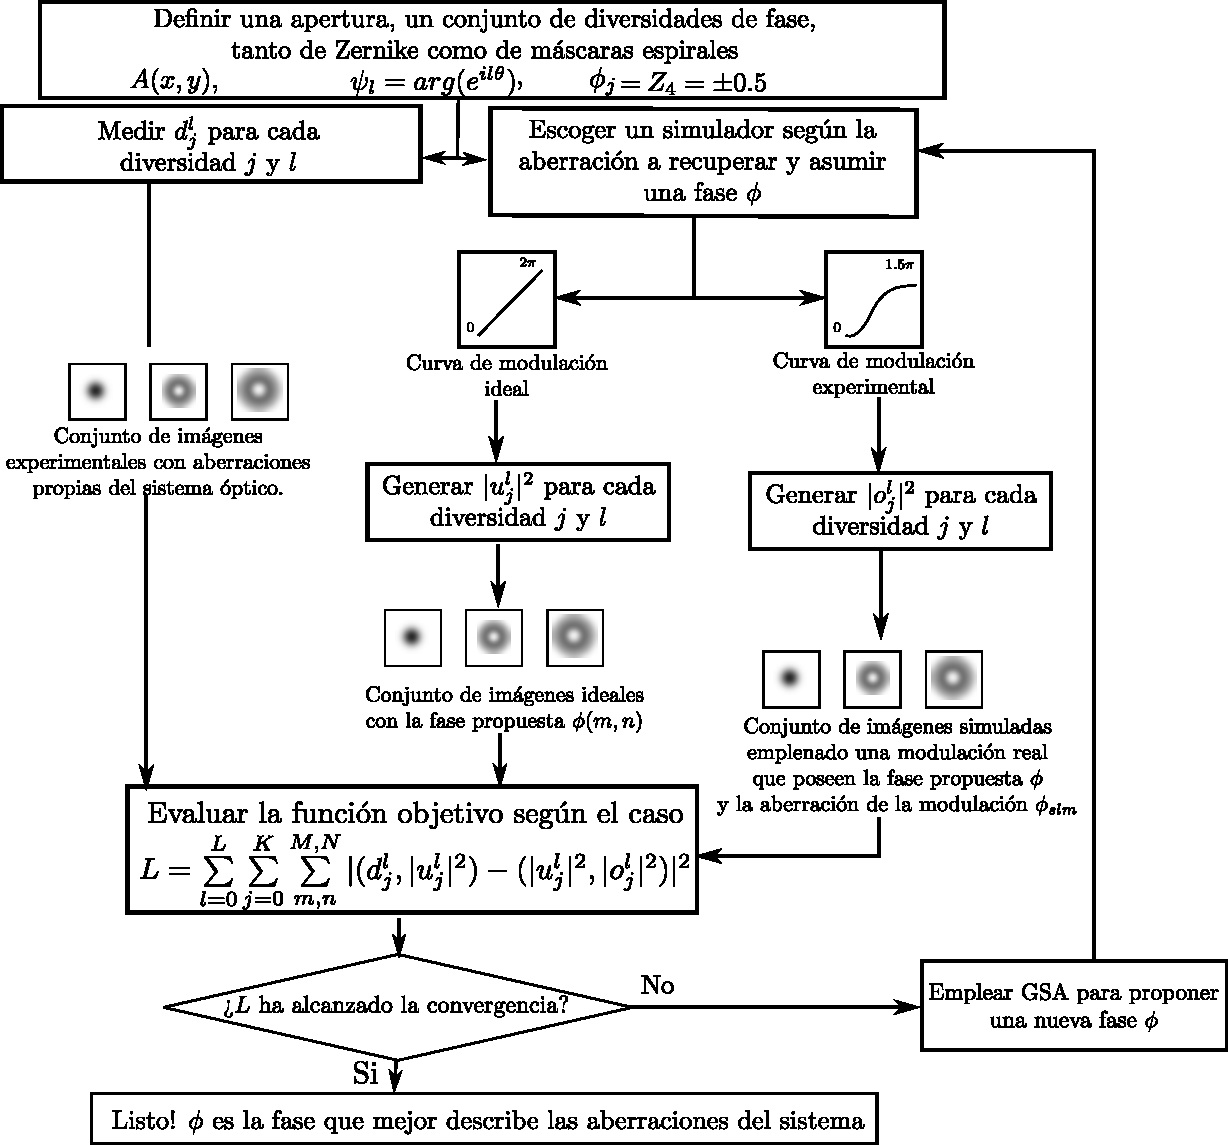
\includegraphics[scale=0.4]{img/pdfluxadd.pdf}
			\end{center}
		\end{frame}	
	
	\subsection{Resultados: Modificaciones sobre PD coherente}
		\begin{frame}
		\frametitle{Diversidad de fase como sensor de aberraciones a causa de la modulación en fase (PD2)}
		\begin{center}
		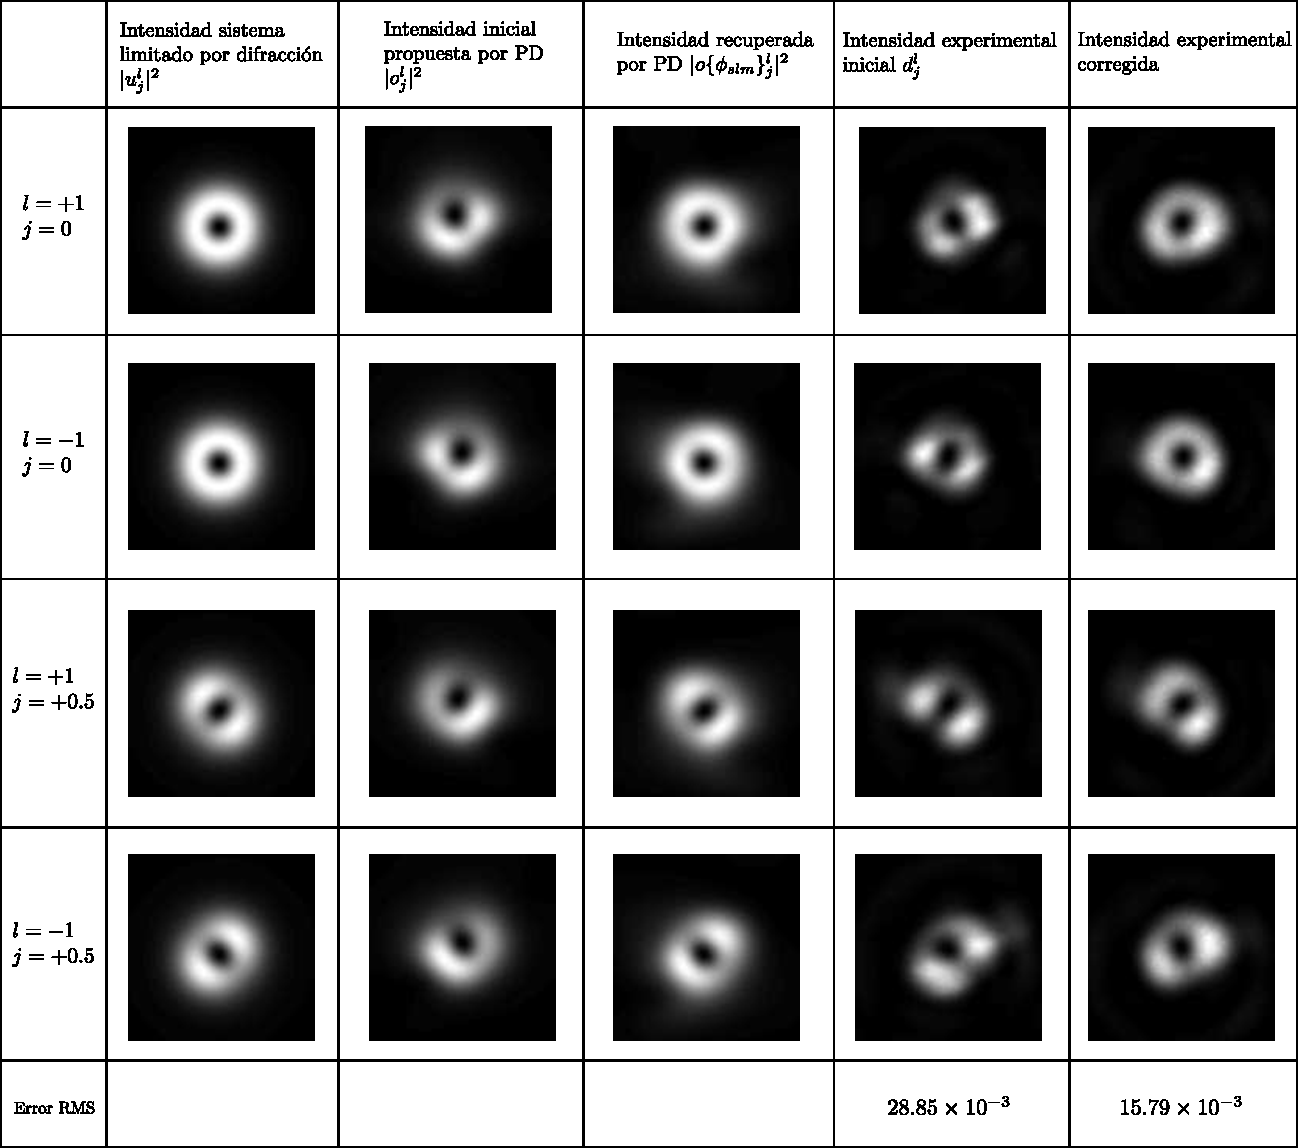
\includegraphics[scale=0.4]{img/CorPD2.pdf}
		\end{center}
		\end{frame}

		\begin{frame}
		\frametitle{Diversidad de fase como sensor de aberraciones a causa del sistema óptico (PD1)}
		\begin{center}		
			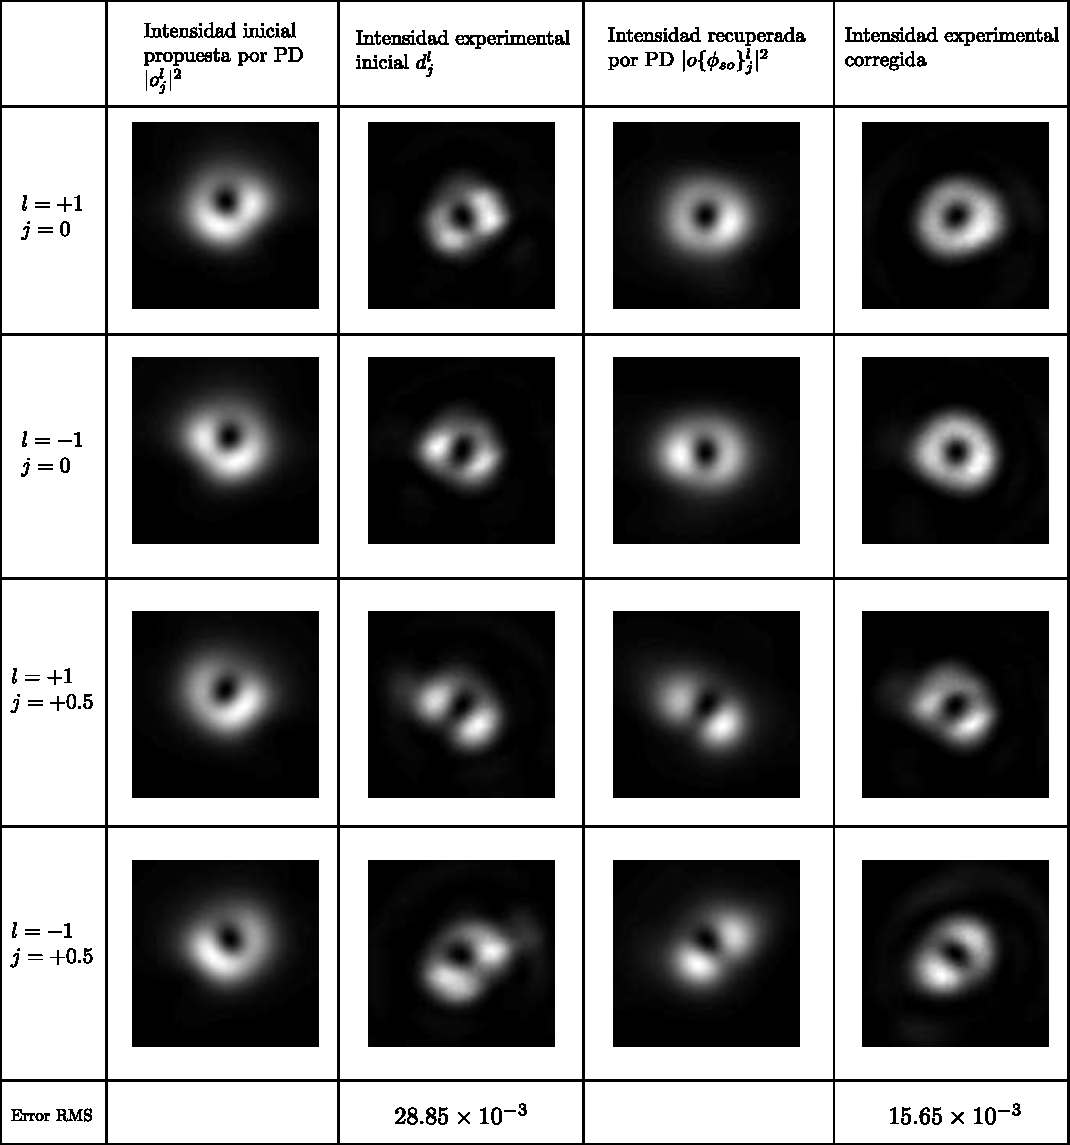
\includegraphics[scale=0.4]{img/CorPD1.pdf}
		\end{center}
		
		\end{frame}

		\begin{frame}
		\frametitle{Recuperación de la aberración causada por el SLM}
			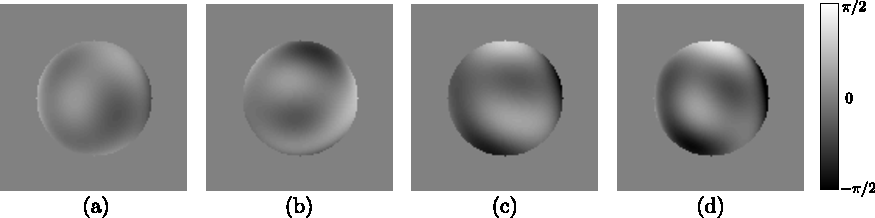
\includegraphics[scale=0.75]{img/fases.pdf}\\
			Comparación de las aberraciones obtenidas para cada una de las modificaciones de PD coherente. (a) Aberración obtenida con PD coherente, (b) aberración obtenida con PD1, (c) aberración obtenida con PD2 y (d) aberración obtenida a través de la diferencia entre (a) y (b).
			\vspace{10pt}
			\begin{center}
			\begin{tabular}{|c|c|}
\hline 
Comparación & Error RMS $[\lambda]$ \\ 
\hline 
(c) - Frente de onda plano & $66.21\times 10^{-3} $ \\ 
\hline 
(d) - Frente de onda plano & $66.31\times 10^{-3}$ \\ 
\hline 
(c) - (d) & $0.87 \times 10^{-3}$ \\ 
\hline 
\end{tabular}
			\end{center}

		\end{frame}
%		
%%%%%%% SECCIÓN: CONCLUSIONES %%%%%
\section{Conclusiones}
	\setcounter{subsection}{1}
	
	%%% Conclusiones %%%
	%\subsection{Conclusiones}
		\begin{frame}
		\frametitle{Conclusiones}
			\begin{itemize}
			\justifying
			\item El mejor estado para la generación de OVs no necesariamente es aquel donde la modulación en fase es de $2\pi$ dado que también debe haber un compromiso con la modulación en amplitud.
			\item A partir de la curva de modulación en fase, se implementó un algoritmos para la simulación de los OVs generados con dicha curva de modulación y esta se empleó en algoritmos de diversidad de fase.
			\item Se propuso una nueva aplicación para PD coherente basado en la curva de modulación que permite determinar las aberraciones que son inducidas por una modulación en fase no ideal.
			\item Se obtuvo las aberraciones de un sistema óptico, diferenciando en estas aquellas que son producidas por el SLM y por los demás elementos ópticos.
			\item Se comprobó la validez del método recuperando las aberraciones causadas por la modulación del SLM a través de las del sistema óptico y las totales obtenidas.
			\end{itemize}
		\end{frame}
		
		\begin{frame}
		\frametitle{Trabajo futuro}
		\begin{itemize}
		\item Emplear vórtices ópticos generados mediante redes de difracción en los algoritmos de diversidad de fase propuestos.
		\item Implementar PD2 para la detección de aberraciones ocasionadas por la modulación de fase de un SLM diferente.
		\item Estudiar la generación de vórtices ópticos con iluminación parcialmente coherente y desarrollar un algoritmo de diversidad de fase para este caso.

		\end{itemize}
		\end{frame}
%
%%%%%%% SECCIÓN AGRADECIMIENTOS %%%%%
%%\begin{frame}
%%\frametitle{Agradecimientos}
%%	Aquí van los agradecimientos a toute le monde
%%\end{frame}
%
%%%%%%%%% Página final %%%%%%%%
\setbeamertemplate{headline}{}
\setbeamertemplate{logo}{}
\begin{frame}
\vfill
\centering
\huge ¿Alguna pregunta?\\

\includegraphics[height=\paperheight,keepaspectratio]{img/Final.eps}
\vfill
\end{frame}

\begin{frame}[allowframebreaks]
\frametitle{Referencias}
%  \begin{frame}[allowframebreaks]
%  \frametitle{Bibliograf\'ia}
\nocite{*}
  \bibliographystyle{unsrt}
  \bibliography{ReferenciasPresentacion}
%  \end{frame}
\end{frame}














%%%%%%%% SECCION: RESULTADOS %%%%%%%%	
%\section{Resultados}
%	\setcounter{subsection}{1}
%
%	%%% Curvas de modulación %%%
%	%\subsubsection{Curvas de modulación experimentales}
%		\begin{frame}
%		\frametitle{Curvas de modulación experimentales}
%			Aquí se pasa el montaje rapidamente
%		\end{frame}
%
%	%%% Simulación de OVs a partir de curvas de modulación %%%
%	\subsection{Simulación de vórtices ópticos a partir de las curvas de modulación}
%		\begin{frame}
%		\frametitle{Generación experimental de vórtices ópticos}
%			Aquí se pasa el montaje rapidamente
%		\end{frame}
%
%	%%% Resultados Caractterización SLM %%%
%	\subsection{Generación experimental de vórtices ópticos}
%		\begin{frame}
%		\frametitle{Generación experimental de vórtices ópticos}
%			Aquí se pasa el montaje rapidamente
%		\end{frame}
%	
%	%%% Resultados corrección con PD coherente %%%
%	\subsection{Correcciones con diversidad de fase coherente}
%		\begin{frame}
%		\frametitle{Correcciones con diversidad de fase coherente}
%			Aquí se pasa el montaje rapidamente
%		\end{frame}
%		
%	%%% PD como sensor de aberraciones a causa de modulación en fase %%%
%	%\subsubsection{Diversidad de fase como sensor de aberraciones a causa de la modulación en fase}
%		\begin{frame}
%		\frametitle{Diversidad de fase como sensor de aberraciones a causa de la modulación en fase}
%			Aquí se pasa el montaje rapidamente
%		\end{frame}
%
%	%%% PD como sensor de aberraciones de sistema óptico %%%
%	%\subsubsection{Diversidad de fase como sensor de aberraciones a causa del sistema óptico}
%		\begin{frame}
%		\frametitle{Diversidad de fase como sensor de aberraciones a causa del sistema óptico}
%			Aquí se pasa el montaje rapidamente
%		\end{frame}
		
	%%% Recuperación de la aberración de modulacón a partir de los resultados anteriores %%%
	%\subsection{Recuperación de la aberración de modulación a partir de las aberraciones del sistema óptico}
%		\begin{frame}
%		\frametitle{Montaje experimental}
%			Aquí se pasa el montaje rapidamente
%		\end{frame}
		







%%%%%%%%% SECCION: IMPLEMENTACIONES %%%%%%%%	
%\section{Implementaciones experimentales}
%	\setcounter{subsection}{1}
%
%	%%% Caracterizacion SLM %%%
%	\subsection{Caracterización del modulador espacial de luz}
%		\begin{frame}
%		\frametitle{Caracterización del modulador espacial de luz}
%			Aquí van los rotadores y la tesis del jefe.
%		\end{frame}
%
%	%%% Mask app %%%
%	\subsection{Programa para la presentación de máscaras al SLM}
%		\begin{frame}
%		\frametitle{Programa para la presentación de máscaras al SLM}
%			Aquí se pasa el montaje rapidamente
%		\end{frame}
%	
%	%%% Montaje Experimental %%%
%	\subsection{Montaje experimental}
%		\begin{frame}
%		\frametitle{Montaje experimental}
%			Aquí se pasa el montaje rapidamente
%		\end{frame}









%%%%% Introducción %%%%%
%\section{Introducción} 
%\setcounter{subsection}{1}
%
%	\subsection{Vórtice óptico}
%		\begin{frame} 
%		\frametitle{Vórtice óptico}
%		Un vórtice óptico (VO) es una dislocación del frente de onda que genera una singularidad en la fase y causa un punto de intensidad nula. 
%		\footnote{M. R. Dennis, K. O’Holleran, and M. J. Padgett. ``Chapter 5 singular optics: Optical vortices and polarization singularities''. Progress in Optics, volumen 53, páginas 293–363. Elsevier, 2009.} 
%		
%		Su función de onda depende de la distribución espacial del frente de onda de forma que la fase es proporcional al plano azimutal
%		\begin{equation}
%		\psi(x,y) \propto e^{qi\theta(x,y)},
%		\end{equation}
%		donde $q$ es un entero conocido como carga topológica y, 		$$\theta(x,y) = \arctan\left(\frac{y}{x}\right)$$
%		\begin{figure}
%		\includegraphics[scale=0.3]{dibujo.png}
%		\caption{A) Vórtice óptico, B) perfil de fase azimutal $\theta$ y C) propagación de la fase.}
%		\end{figure}	
%		\end{frame}
%		
%	\subsection{Generación de vórtices ópticos}
%		\begin{frame}
%		\frametitle{Generación de vórtices ópticos}
%		\begin{multicols}{3}
%			\vfill
%			\centering Manipulación controlada de las propiedades de los láseres\footnote{T. Ohtomo, S. Chu, and K. Otsuka. ``Generation of vortex beams from lasers with controlled herte- and ince- gaussian modes''. Optics Express,
%\textbf{16}(7), 5082–5094 (2008).}.
%			\begin{figure}
%			\includegraphics[scale=0.25]{LGmodos.pdf}
%			\caption{Modos Laguerre-Gauss}
%			\end{figure}
%			\vfill
%			
%			\newpage
%			\vfill
%			\centering Empleando placas espirales de fase (SPP)\footnotemark[1]. 
%			\begin{figure}
%			\includegraphics[scale=0.25]{SPP.eps}
%			\caption{VO a partir de SPP. }
%			\end{figure}
%			
%			\newpage 
%			\vfill
%			\centering Empleando elementos difractivos\footnotemark[1].
%			\begin{figure}
%			\includegraphics[scale=0.25]{DiffGrat.eps}
%			\caption{VO a partir de redes de difracción.}
%			\end{figure}
%		\end{multicols}
%		\end{frame}
%		
%	\subsection{Modulador espacial de luz}
%		\begin{frame}
%		\frametitle{Modulador espacial de luz}
%		Dispositivos que modulan amplitud o fase de ondas de luz en espacio y tiempo. \footnote{HOLOEYE Photonics. \url{http://holoeye.com/spatial-light-modulators/}}.
%		
%		\begin{figure}
%		\includegraphics[scale=0.4]{Mod.eps}
%		\caption{Moduladores espaciales de luz.\footnotemark[3]}
%		\end{figure}
%		\end{frame}
%		
%\setbeamertemplate{logo}{}
%	
%	\subsection{¿Por qué redes de difracción?}
%		\begin{frame}
%		\frametitle{¿Por qué redes de difracción?}
%		
%		\begin{figure}
%		\includegraphics[scale=0.3]{ovsimreal.pdf}
%		\caption{Efectos de modulación no ideal sobre VO.}
%		\end{figure}
%		
%		\begin{multicols}{2}
%		
%		\begin{itemize}
%		\item Efectos de modulaciones de fase no ideales menos representativos.
%		\item Empleo del SLM en configuraciones de amplitud.
%		%\item Menor sensibilidad ante aberraciones.
%		\end{itemize}
%		
%		\newpage
%		\centering
%		\begin{figure}
%		\includegraphics[scale=0.4]{BinProfile.pdf}
%		\caption{Red binaria ``bifurcada''.}
%		\end{figure}
%		
%		\end{multicols}
%		
%		\end{frame}
%\setbeamertemplate{logo}{\includegraphics[scale=0.15]{logoeafit.png}\vspace{0pt}}
%
%	\subsection{Análisis desde la óptica de Fourier}
%		\begin{frame}
%		\frametitle{Análisis desde la óptica de Fourier}
%
%		\begin{figure}
%		\includegraphics[scale=0.4]{BlackBox.eps}
%		\caption{Modelo ``caja negra''.}
%		\end{figure}		
%		
%		Para el caso de un sistema óptico con iluminación coherente \footnote{\tiny D. Voelz. ``Computational Fourier Optics''. SPIE PRESS, 2011.} \footnote{\tiny J. Goodman. ``Introduction to Fourier Optics''. McGraw-Hill, 1996.}
%		\begin{equation}
%		U_{ima} (u,v)= h(u,v) \otimes U_{geo}(u,v),
%		\end{equation}
%		%h(u,v) es la respuesta al impulso coherente
%		donde $$U_{geo} (u,v) = \frac{1}{|M_t|} U_{obj} \left(\frac{u}{M_t},\frac{v}{M_t}\right).$$
%		Empleando el teorema de la convolución y transformadas de Fourier
%		\begin{equation}
%		U_{ima} (u,v) = \mathscr{F}^{-1}\{ H(f_u,f_v) \mathscr{F}\{U_{geo}(u,v)\} \},
%		\end{equation}
%		$H(f_u,f_v)$ es la función de transferencia de amplitud
%		\begin{equation}
%		H(f_u,f_v) = P(x,y) e^{jW(x,y)}.
%		\end{equation}
%		
%		\end{frame}
%		
%	\subsection{¿Cómo se hace experimentalmente?}
%		\begin{frame}
%		\frametitle{¿Cómo se hace experimentalmente?}
%		A partir de un correlador $4F$.
%		\begin{figure}
%		\includegraphics[scale=0.55]{4F.pdf}
%		\caption{Sistema $4F$.}
%		\end{figure}
%		\end{frame}
%				
%%%%%%% Planteamiento del Problemo %%%%%%
%\section{Planteamiento del problema}
%\setcounter{subsection}{1}
%\begin{frame} \frametitle{Planteamiento del problema}
%El problema central de este proyecto es la obtención de vórtices ópticos a partir de un modulador espacial de luz de transmisión empleando tres tipos de redes de difracción: binaria, sinusoidal y diente de sierra.
%\end{frame}
%
%%%%%%% Objetivos %%%%%%
%\section{Objetivos}
%\setcounter{subsection}{1}
%\begin{frame} \frametitle{Objetivos}
%
%\subsubsection{General}
%	\begin{block}{General}
%		Simular y comparar con resultados experimentales vórtices ópticos generados a través de redes de difracción.
%	\end{block}
%
%\subsubsection{Específicos}
%\begin{block}{Específicos}
%	\begin{itemize}
%		\item Simular la propagación de frentes de onda a través de redes de difracción del tipo binaria, sinusoidal y diente de sierra sumadas a una máscara espiral de fase.
%
%		\item Comparar por medio de simulaciones las tres redes de difracción ante la presencia de aberraciones ópticas en la formación de vórtices ópticos.
%
%		\item Implementar una interfaz gráfica para la generación de redes de difracción para ser proyectadas en un modulador espacial de luz.
%
%		\item Obtener resultados experimentales para cada red de difracción mediante el empleo de un modulador espacial de luz.
%
%		\item Comparar los resultados de las simulaciones con los resultados experimentales.
%	\end{itemize}
%\end{block}
%\end{frame}
%
%% No hay tiempo para estas mamadas
%%%%%% Metodología %%%%%
%%\section{Metodología}
%%\setcounter{subsection}{1}
%%	\begin{frame} 
%%	\frametitle{Metodología}
%%	
%%	\end{frame}
%
%%%%%% Avances %%%%%
%\section{Resultados}
%\setcounter{subsection}{1}
%\begin{frame} 
%	\frametitle{Resultados: \\ \hspace{10pt} -Generación de las máscaras}
%	\begin{figure}
%	\centering \includegraphics[scale=0.9]{redes.pdf}
%	\caption{Generación de las máscaras diente de sierra, binarias y sinusoidales.}
%	\end{figure}
%\end{frame}
%
%\begin{frame} 
%	\frametitle{Resultados: \\ \hspace{10pt} -Algoritmo para la simulación de vórtices ópticos a partir de redes de difracción.}
%	\begin{figure}
%	\centering \includegraphics[scale=0.8]{GenVor.pdf}
%	\caption{Algoritmo para simular la generación de vórtices ópticos a partir de redes de difracción.}
%	\end{figure}
%\end{frame}
%
%\begin{frame}
%	\frametitle{Resultados: \\ \hspace{10pt} -Simulación de propagación por redes de difracción con diferente periodo}
%		\begin{figure}
%		\centering \includegraphics[scale=0.5]{OvsSimFin.pdf}
%		\caption{Simulación de la propagación cuando se varía el periodo de la red de difracción.}
%		\end{figure}
%\end{frame}
%
%\begin{frame}
%	\frametitle{Resultados: \\ \hspace{10pt} -Simulación de propagación con aberraciones}
%		\begin{figure}
%		\centering \includegraphics[scale=0.7]{AberraComp.pdf}
%		\caption{Simulación de la propagación cuando se presentan aberraciones en las redes de difracción.}
%		\end{figure}
%\end{frame}
%%
%%\setbeamertemplate{logo}{}
%\begin{frame}
%	\frametitle{Resultados: \\ \hspace{10pt} -Interfaz gráfica para la presentación de máscaras al SLM.}
%	
%	\begin{figure}
%	\begin{center}
%	\includegraphics[scale=0.4]{MaskAppEspec.pdf}
%	\caption{Interfaz gráfica implementada.}
%	\end{center}
%	\end{figure}
%	
%\end{frame}
%
%%\begin{frame}
%%
%%	\frametitle{Resultados: \\ \hspace{10pt} -Montaje experimental.}
%%
%%%\begin{figure}[!ht]
%%  \centering
%%    \includegraphics[width=\textwidth,keepaspectratio]{Montaje.pdf}
%%  \caption{Esquema del montaje experimental.}
%%  \label{fig:montaje}
%%\end{figure}
%%\end{frame}
%%\begin{frame}
%%
%%	\frametitle{Resultados: \\ \hspace{10pt} -Montaje experimental.}
%%\begin{figure}[!ht]
%%  \centering
%%    \includegraphics[width=\textwidth,keepaspectratio]{montexp.JPG}
%%  \caption{Montaje experimental.}
%%  \label{fig:montexp}
%%\end{figure}
%%
%%\end{frame}
%%\setbeamertemplate{logo}{}
%%\setbeamertemplate{logo}{\includegraphics[scale=0.15]{logoeafit.png}\vspace{0pt}}
%
%\begin{frame}
%	\frametitle{Resultados: \\ \hspace{10pt} -Vórtices ópticos experimentales}
%		\begin{figure}
%		\centering \includegraphics[scale=0.5]{OVExpNoAB.pdf}
%		\caption{Comparación entre VOs simulados y obtenidos experimentalmente.}
%		\end{figure}
%\end{frame}
%
%\begin{frame}
%	\frametitle{Resultados: \\ \hspace{10pt} -Vórtices ópticos ante la presencia de aberraciones en la red}
%		\begin{figure}
%		\centering \includegraphics[scale=0.6]{OVExp.pdf}
%		\caption{Comparación experimental de la propagación cuando se presentan aberraciones en las redes de difracción.}
%		\end{figure}
%\end{frame}
%%%%%% Conclusiones Parciales %%%%%
%\section{Conclusiones}
%\setcounter{subsection}{1}
%\begin{frame} 
%\frametitle{Conclusiones}
%	\begin{itemize}
%		\item Se demostró que las redes de difracción permiten la generación de vórtices ópticos.
%		\item La forma en la cual se a planteado el problema permite el análisis de este desde una perspectiva de la óptica de Fourier.
%		\item Se pueden generar VO a partir de redes de difracción en configuraciones de amplitud.
%		\item Las redes binarias pueden emplearse tanto en fase como en amplitud y en esta última, su comportamiento es similar a una red sinusoidal.
%		\item Los vórtices ópticos obtenidos poseen una simetría en la carga topológica, como la que presentan los ordenes difractados.
%		\item Pueden agregarse aberraciones a redes de difracción, de forma que estas se reflejan en una deformación de la red.
%	\end{itemize}
%\end{frame}
%
%%%%%% Trabajo futuro %%%%%
%\section{Trabajo futuro}
%\setcounter{subsection}{1}
%\begin{frame} \frametitle{Trabajo futuro}
%
%Como trabajo futuro se propone:
%
%\begin{itemize}
%	\item Analizar las efectos de muestreo sobre las redes
%	\item Analizar los efectos de la no idealidad del SLM sobre los VO.
%	\item Implementar redes de difracción en algoritmos de diversidad de fase coherente.
%\end{itemize}
%\end{frame}

%%%%% Bibliografía si necesario %%%%%
%\section{Bibliografía o no}
%\setcounter{subsection}{1}
%\begin{frame}
%le bib
%\end{frame}
%\setbeamertemplate{headline}{}
%\begin{frame}
%\vfill
%\centering
%\huge ¡Gracias!\\
%\includegraphics[height=\paperheight,keepaspectratio]{Final.eps}
%\vfill
%\end{frame}

\end{document}
